\documentclass[12pt, a4paper]{article}

\usepackage{array}
\usepackage[portuguese]{babel}
\usepackage{float}
\usepackage[a4paper, margin=2cm]{geometry}
\usepackage{graphicx}
\usepackage{hyperref}
\usepackage{pdfpages}
\usepackage{setspace}

\title{\textbf{Interface Pessoa-Máquina \\ \large Trabalho Prático -- Fase I}}
\date{16 de março de 2025}
\author{Grupo 12 \\
    \url{https://www.figma.com/design/Ps4VLCPz66bKq5p2ypzrDR/Projeto-IPM}}

\begin{document}

\begin{center}
    
\includegraphics[width=0.25\textwidth]{res/cover/school-of-engineering.eps}
\end{center}

{\let\newpage\relax\maketitle}
\maketitle
\thispagestyle{empty}

\chardef\_=`_
\onehalfspacing
\setlength{\parskip}{\baselineskip}
\setlength{\intextsep}{2\baselineskip}
\setlength\belowcaptionskip{-\baselineskip}
\setlength{\parindent}{0pt}
\def\arraystretch{1.5}

\vspace{2cm}
\begin{center}
    \begin{tabular}{>{\centering}p{0.25\textwidth}
                    >{\centering}p{0.25\textwidth}
                    >{\centering\arraybackslash}p{0.25\textwidth}}
        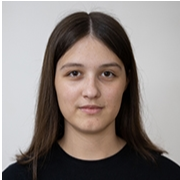
\includegraphics[width=3.5cm]{res/cover/A104437.png} &
        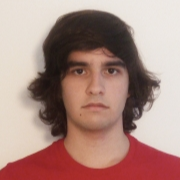
\includegraphics[width=3.5cm]{res/cover/A104348.png} &
        
\includegraphics[width=3.5cm]{res/cover/A104263.png}  \\

        Ana Oliveira & Humberto Gomes & Inês Marques \\
        A104437      & A104348        & A104263
    \end{tabular}

    \begin{tabular}{>{\centering}p{0.25\textwidth}
                    >{\centering\arraybackslash}p{0.25\textwidth}}
        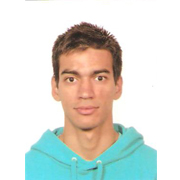
\includegraphics[width=3.5cm]{res/cover/A76350.jpg} &
        
\includegraphics[width=3.5cm]{res/cover/A104179.png} \\

        Rafael Vilas Boas & Sara Lopes \\
        A76350            & A104179
    \end{tabular}
\end{center}

\begin{abstract}
    \noindent
    No âmbito deste trabalho prático, foi prototipada uma interface de utilizador de um sistema para
    a gestão de horários de um curso universitário, utilizado tanto pelos alunos como pelo diretor
    de curso. Neste documento, apresenta-se a interface modelada com recurso à ferramenta Figma
    \cite{figma}, justificando as várias decisões tomadas face aos perfis dos utilizadores da
    aplicação. Perante o grande volume de dados que são horários, o principal foco do
    desenvolvimento desta interface foi a apresentação desta informação de uma forma familiar,
    flexível, e sem sobrecarregar o utilizador. Foi também realizada uma avaliação da interface
    apresentada, fazendo uso das heurísticas de Nielsen \cite{nielsen}. Apesar de algumas limitações
    da ferramenta de modelação, julga-se ter construído um protótipo de uma interface que cumpre os
    objetivos do enunciado, e que se encontra suficientemente detalhado para a sua implementação.
\end{abstract}

\section{Análise da Interface Desenvolvida}

\subsection{Página ``Iniciar Sessão''}

A primeira página construída foi a página de início de sessão, que é apresentada ao utilizador
quando este abre a aplicação. Nesta página, tal como descrito nos cenários 1 e 4, tanto o diretor
de curso como as alunos inserem as suas credenciais para se autenticarem:

\begin{figure}[H]
    \centering
    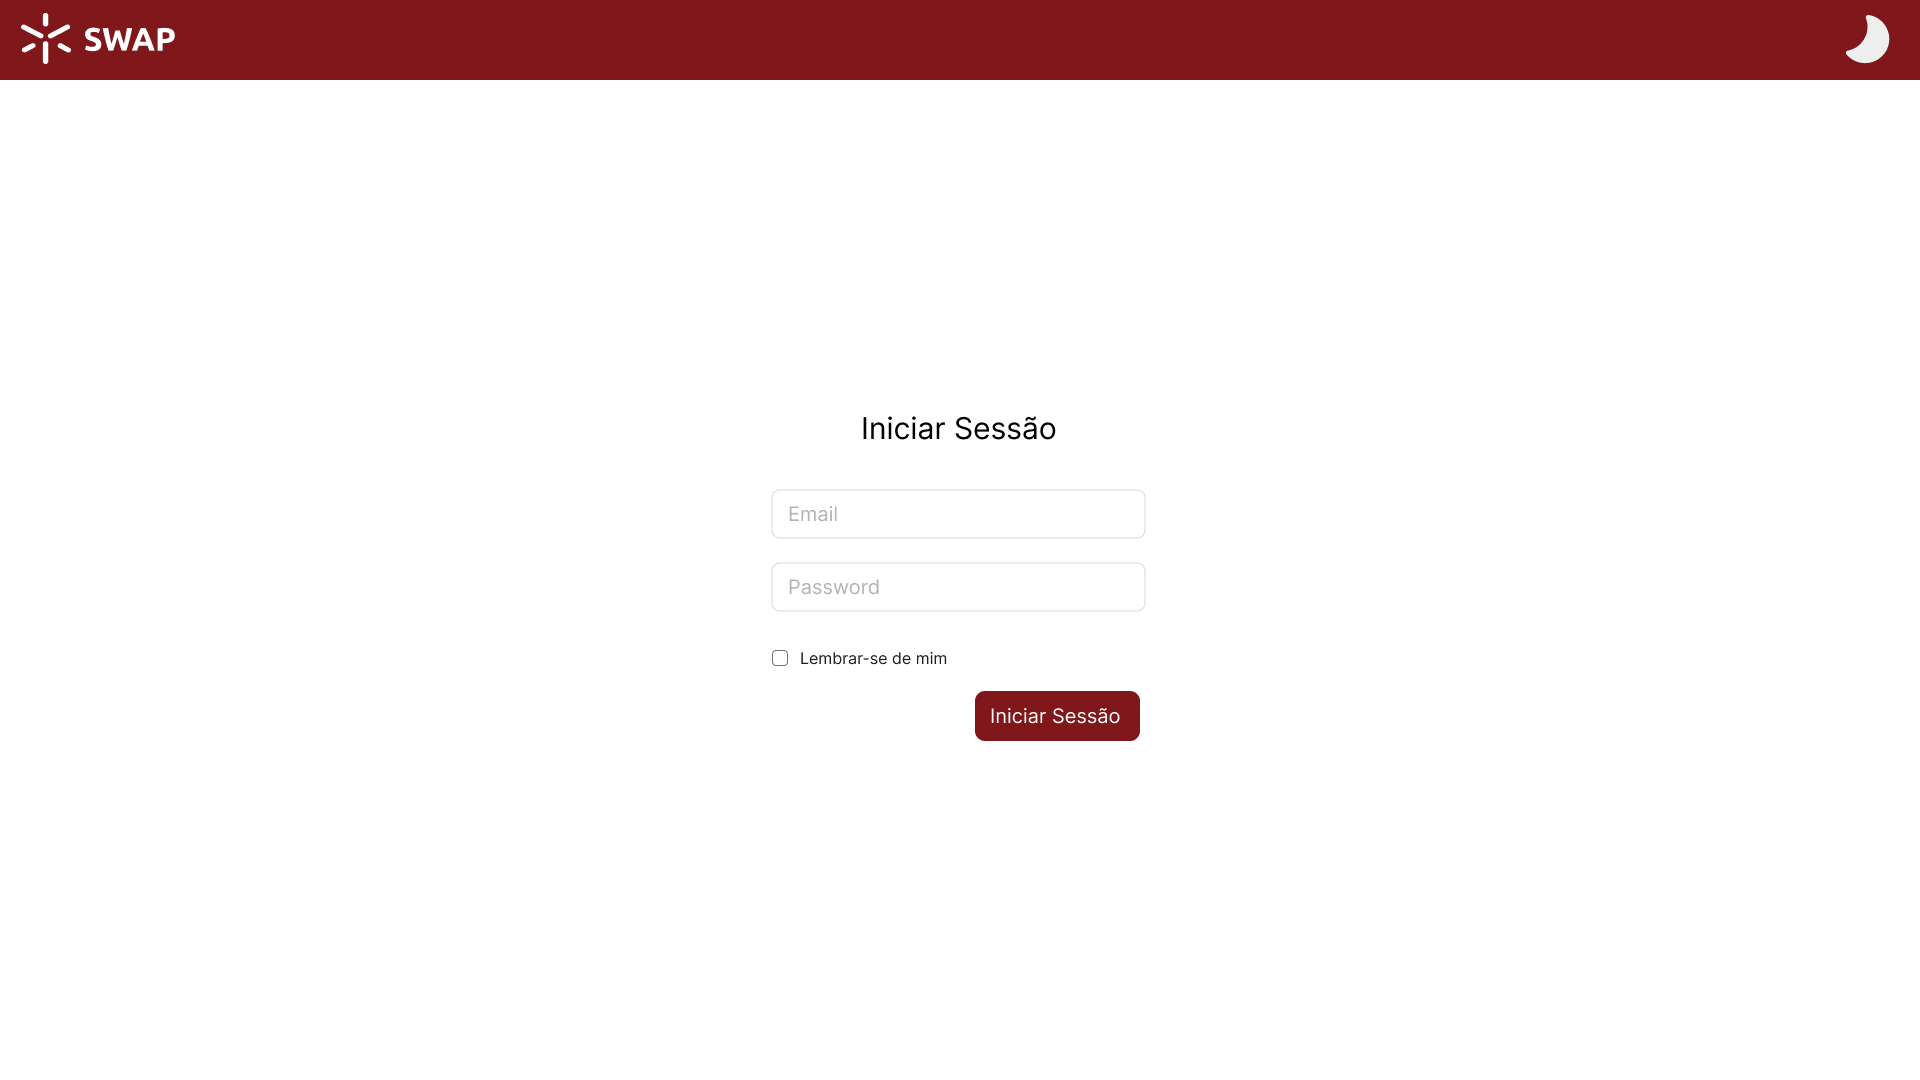
\includegraphics[width=0.8\textwidth]{res/prototype/iniciar-sessao.png}
    \caption{Captura de ecrã do protótipo da página ``Iniciar Sessão'' no tema claro.}
    \label{iniciar-sessao}
\end{figure}

Como não há nada de inovador nesta página, procurou-se inspiração em páginas de início de sessão de
diversos outros \emph{websites}, para se desenvolver uma interface consistente com o que o
utilizador já pode estar familiarizado. Logo, a página é constituída por um título, ``Iniciar
Sessão'', e dois campos de texto explicados com \emph{placeholders}, indicando que informação o
utilizador deve inserir (o seu endereço eletrónico e a sua palavra-passe).

O utilizador também pode escolher se o sistema deve ou não perguntar pelas suas credenciais de
\emph{login} no próximo acesso à aplicação. Caso se opte que o sistema se ``lembre do utilizador'',
é possível poupar algum tempo em usos futuros e recorrentes da aplicação, algo especialmente
importante para o perfil do diretor de curso, que deseja minimizar o seu tempo gasto na gestão de
horários. No entanto, por motivos de segurança, por exemplo, quando a aplicação é utilizada num
computador partilhado, deverá ser possível impedir que o sistema permita o acesso a utilizadores
antes deles providenciarem as suas credenciais.

O perfil da Maria corresponde ao de uma aluna de informática. Apesar de não constar no enunciado, é
de conhecimento geral que muitos dos alunos deste curso não apreciam interfaces em tons claros. Por
este motivo, procurando desenvolver-se uma interface customizável, também se prototipou uma variante
desta interface em tons escuros, que se apresenta abaixo:

\begin{figure}[H]
    \centering
    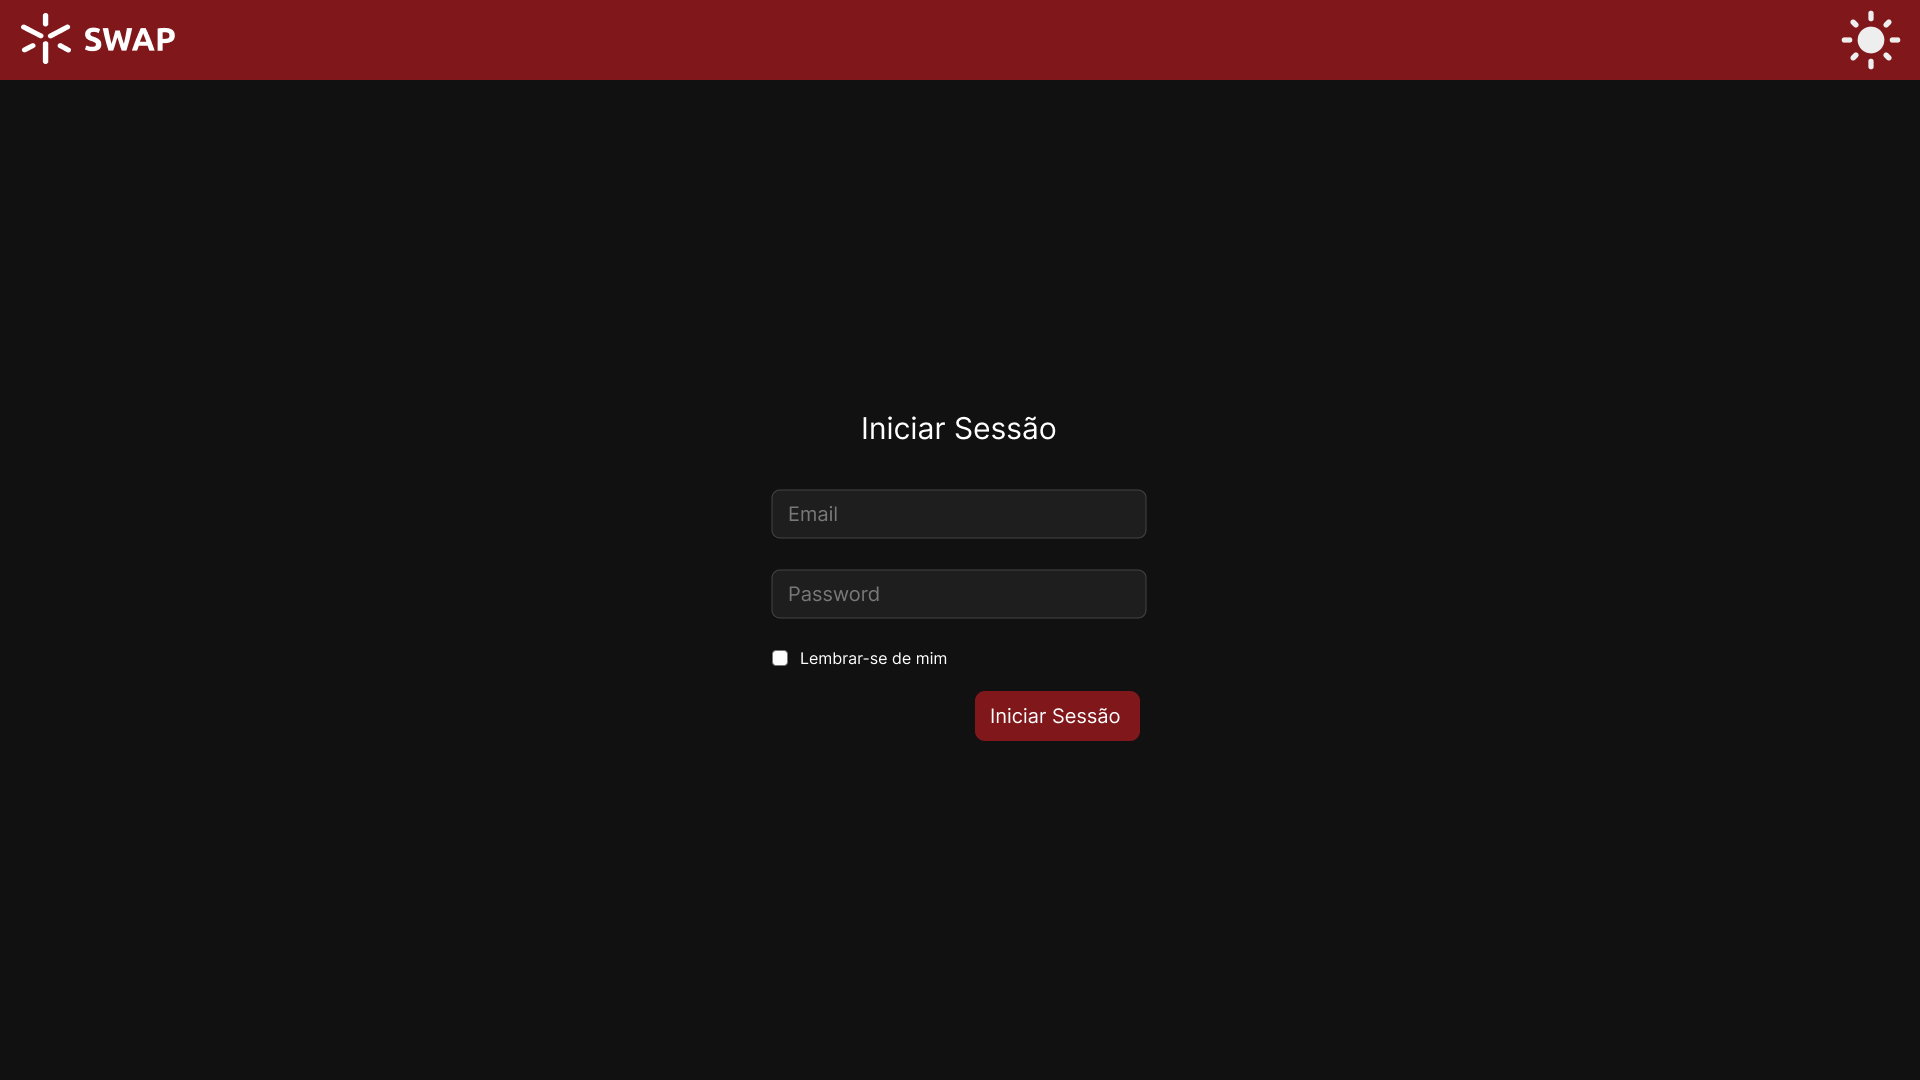
\includegraphics[width=0.8\textwidth]{res/prototype/iniciar-sessao-dark.png}
    \caption{Captura de ecrã do protótipo da página ``Iniciar Sessão'' no tema escuro.}
    \label{iniciar-sessao-dark}
\end{figure}

Visto que o objetivo deste trabalho prático é a prototipagem da estrutura e da funcionalidade da
interface, e não da sua aparência, apenas se prototipou esta página em modo escuro. Para alternar
entre estes dois estilos da aplicação, está sempre disponível um ícone na barra de navegação, uma
lua para ir de modo claro para modo escuro, e um sol para o inverso. Para indicar que é possível
clicar nestes ícones, o seu tom muda quando o utilizador move o cursor para cima dos mesmos. Apesar
de se ter utilizado uma iconografia presente em diversas outras interfaces, Material Icons
\cite{material-icons}, após sobrevoar um ícone com o cursor por algum tempo, uma \emph{tooltip} deve
aparecer, descrevendo o ícone em palavras ao utilizador. Devido a limitações do Figma, não foi
possível prototipar esta funcionalidade. Porém, segue, abaixo, uma simulação visual da aparência
desta \emph{tooltip}:

\begin{figure}[H]
    \centering
    
\includegraphics[width=0.3\textwidth]{res/prototype/icon-tooltip.png}
    \caption{\emph{Tooltip} sobre o ícone de mudança para o tema escuro.}
    \label{icon-tooltip}
\end{figure}

\subsection{Página ``O meu Horário''}

Caso seja um aluno a iniciar sessão, será redirecionado para a página ``O meu Horário'', onde o seu
horário lhe é apresentado, como descreve o cenário 4. Tendo em conta o perfil da utilizadora Maria,
como esta é estudante, assume-se que ela precise de consultar esta página com frequência: para saber
para que sala se deve dirigir no fim de uma aula, que cadernos deve levar na mochila para o dia
seguinte de aulas, \emph{etc.}. Por este motivo, decidiu-se que esta seria a primeira página
apresentada a um estudante depois deste iniciar sessão, pois é a que este mais provavelmente
desejará aceder. Segue-se, abaixo, o protótipo desta página:

\begin{figure}[H]
    \centering
    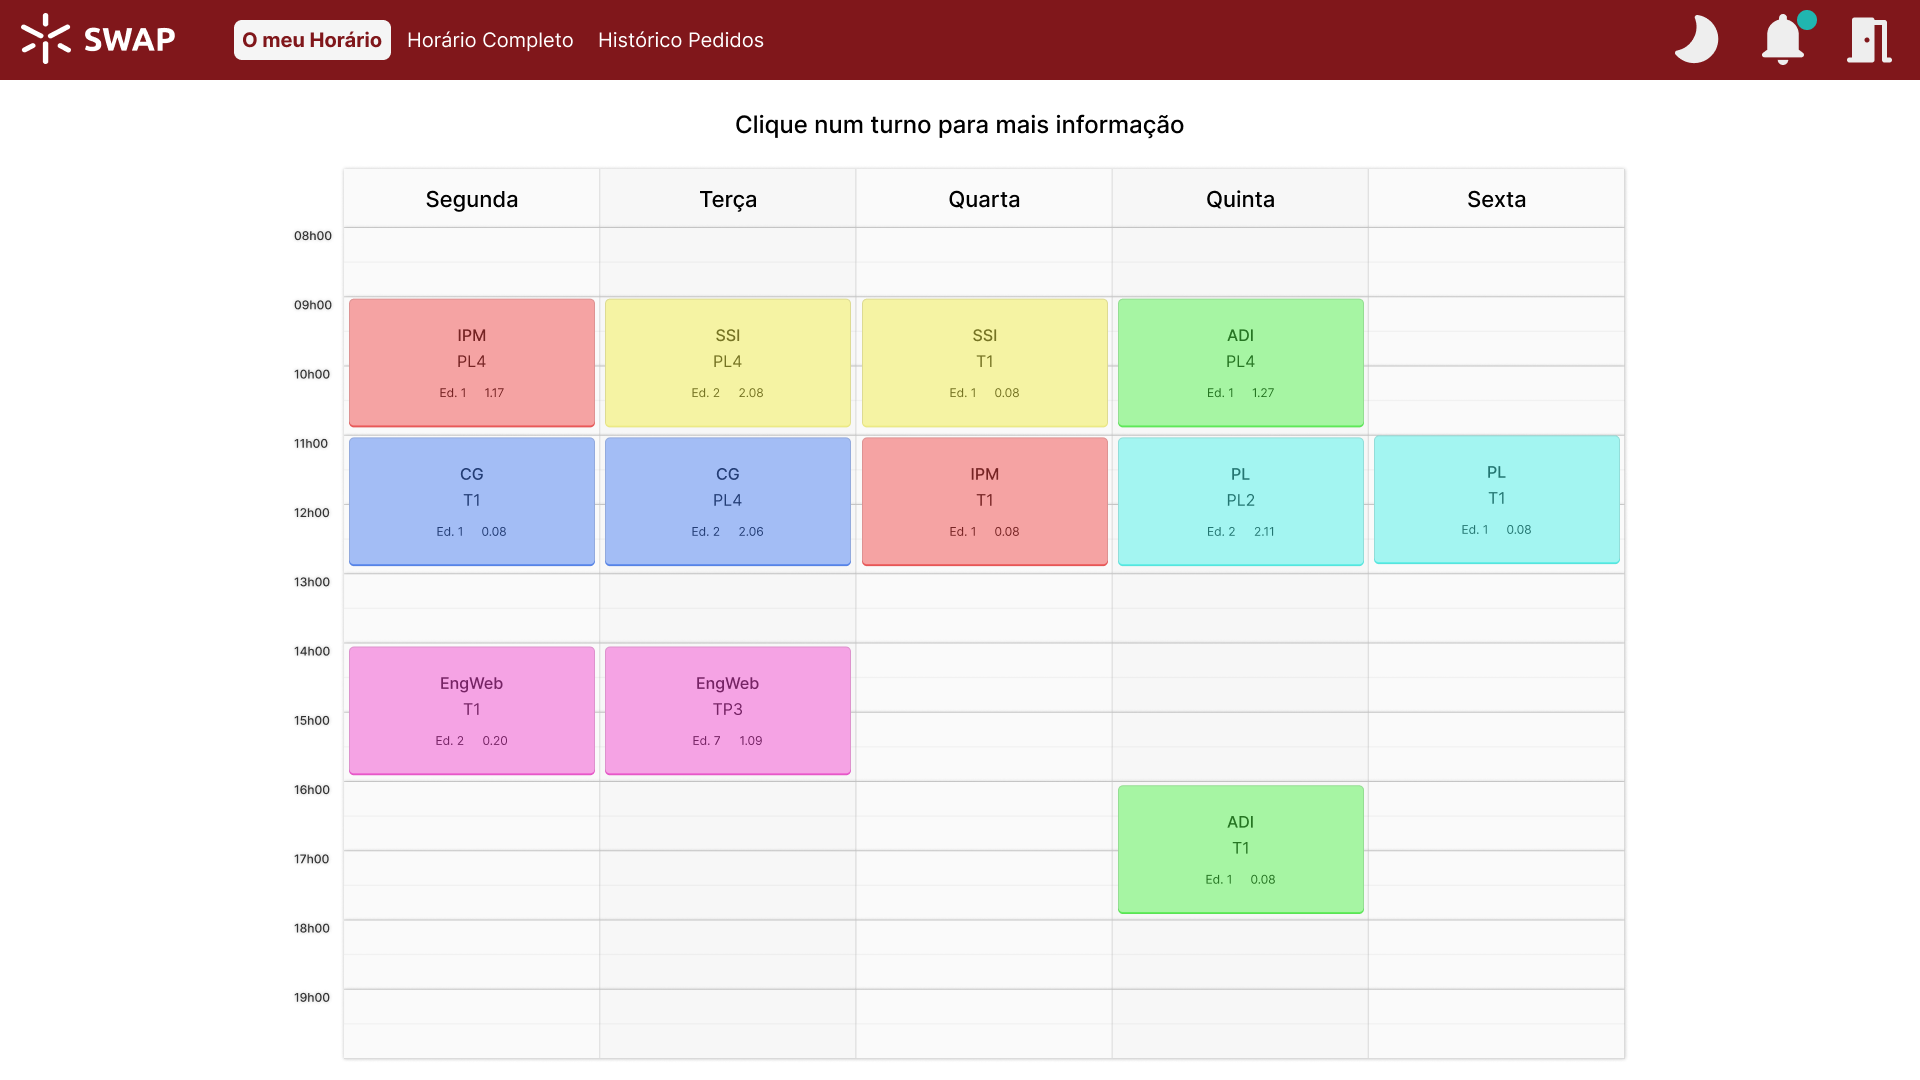
\includegraphics[width=0.8\textwidth]{res/prototype/o-meu-horario.png}
    \caption{Captura de ecrã do protótipo da página ``O meu Horário''.}
    \label{o-meu-horario}
\end{figure}

Antes de justificar a estrutura do conteúdo desta página, é importante explicar o funcionamento da
sua barra de navegação, também presente nas outras páginas às quais os estudantes podem aceder.
Depois do ícone da aplicação, segue uma lista de hiperligações para as páginas acessíveis. A página
onde o utilizador se encontra é realçada com o esquema de cores inverso ao das restantes. Deste
modo, o utilizador sabe sempre em que página se encontra. Do lado direito da barra de navegação,
surgem ícones para trocar o tema da interface (claro ou escuro), ir para a página de notificações, e
para terminar sessão. Novamente, todos estes ícones devem ter uma \emph{tooltip} associada, mesmo
que sejam semelhantes aos utilizados por interfaces de outras aplicações (para uma maior
consistência externa). Para chamar a atenção do utilizador quando há novas notificações, um círculo
surge no canto superior direito do ícone do sino.

O principal elemento do conteúdo da página ``O meu Horário'' é o horário do aluno. Para o apresentar
de uma forma familiar ao utilizador, este é representado como uma grelha de turnos, com os dias da
semana em colunas e as horas do dia em linhas. Os turnos são posicionados nesta grelha conforme a
sua localização temporal. Adicionalmente, para ser fácil que o utilizador distinga entre turnos
diferentes UCs, é associada uma cor a cada UC.

É possível clicar num turno para abrir um diálogo com mais informação. Para ser observável que esta
ação é possível, sobrevoar o cursor a um turno deve mudar a sua cor, e o ícone do cursor deve também
mudar para o do dedo indicador, como mostra a figura abaixo:

\begin{figure}[H]
    \centering
    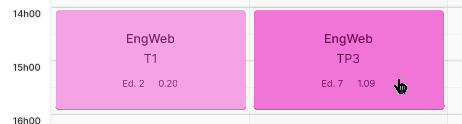
\includegraphics[width=0.6\textwidth]{res/prototype/turno-hover.png}
    \caption{Mudança de cor e de cursor com o sobrevoo do cursor a um turno.}
    \label{turno-hover}
\end{figure}

Mesmo com este efeito, alguns elementos deste grupo de trabalho, também estudantes como a Maria,
tiveram alguma dificuldade em perceber que era possível clicar nos turnos. Ademais, também não
seria possível que utilizadores a utilizar a aplicação sem um rato (por exemplo, com um ecrã tátil)
se apercebessem que era possível interagir com os turnos. Por esse motivo, o texto ``Clique num
turno para mais informação'' foi colocado no topo da página.

Quando o utilizador clica num turno, deve sobrepor-se um diálogo com informação sobre o mesmo, como
mostra a figura abaixo. O fundo da página é escurecido para realçar o diálogo, que mostra mais
detalhes sobre o turno em que o utilizador clicou, como o docente que o leciona e a sua lotação.
Para não sobrecarregar o utilizador com informação na visão normal do seu horário, esta foi colocada
neste diálogo à parte, permitindo uma observabilidade do estado do programa mesmo em ecrãs de
tamanho limitado. É possível fechar este diálogo clicando no ``X'' no seu canto superior direito, o
que é consistente com outras interfaces WIMP (\emph{Windows, Icons, Menus, Pointer}), mas também
clicando fora da sua área (na página ``atrás''), para esta ação ser mais simples para utilizadores
com problemas de destreza manual ou a utilizar ecrãs mais pequenos.

\begin{figure}[H]
    \centering
    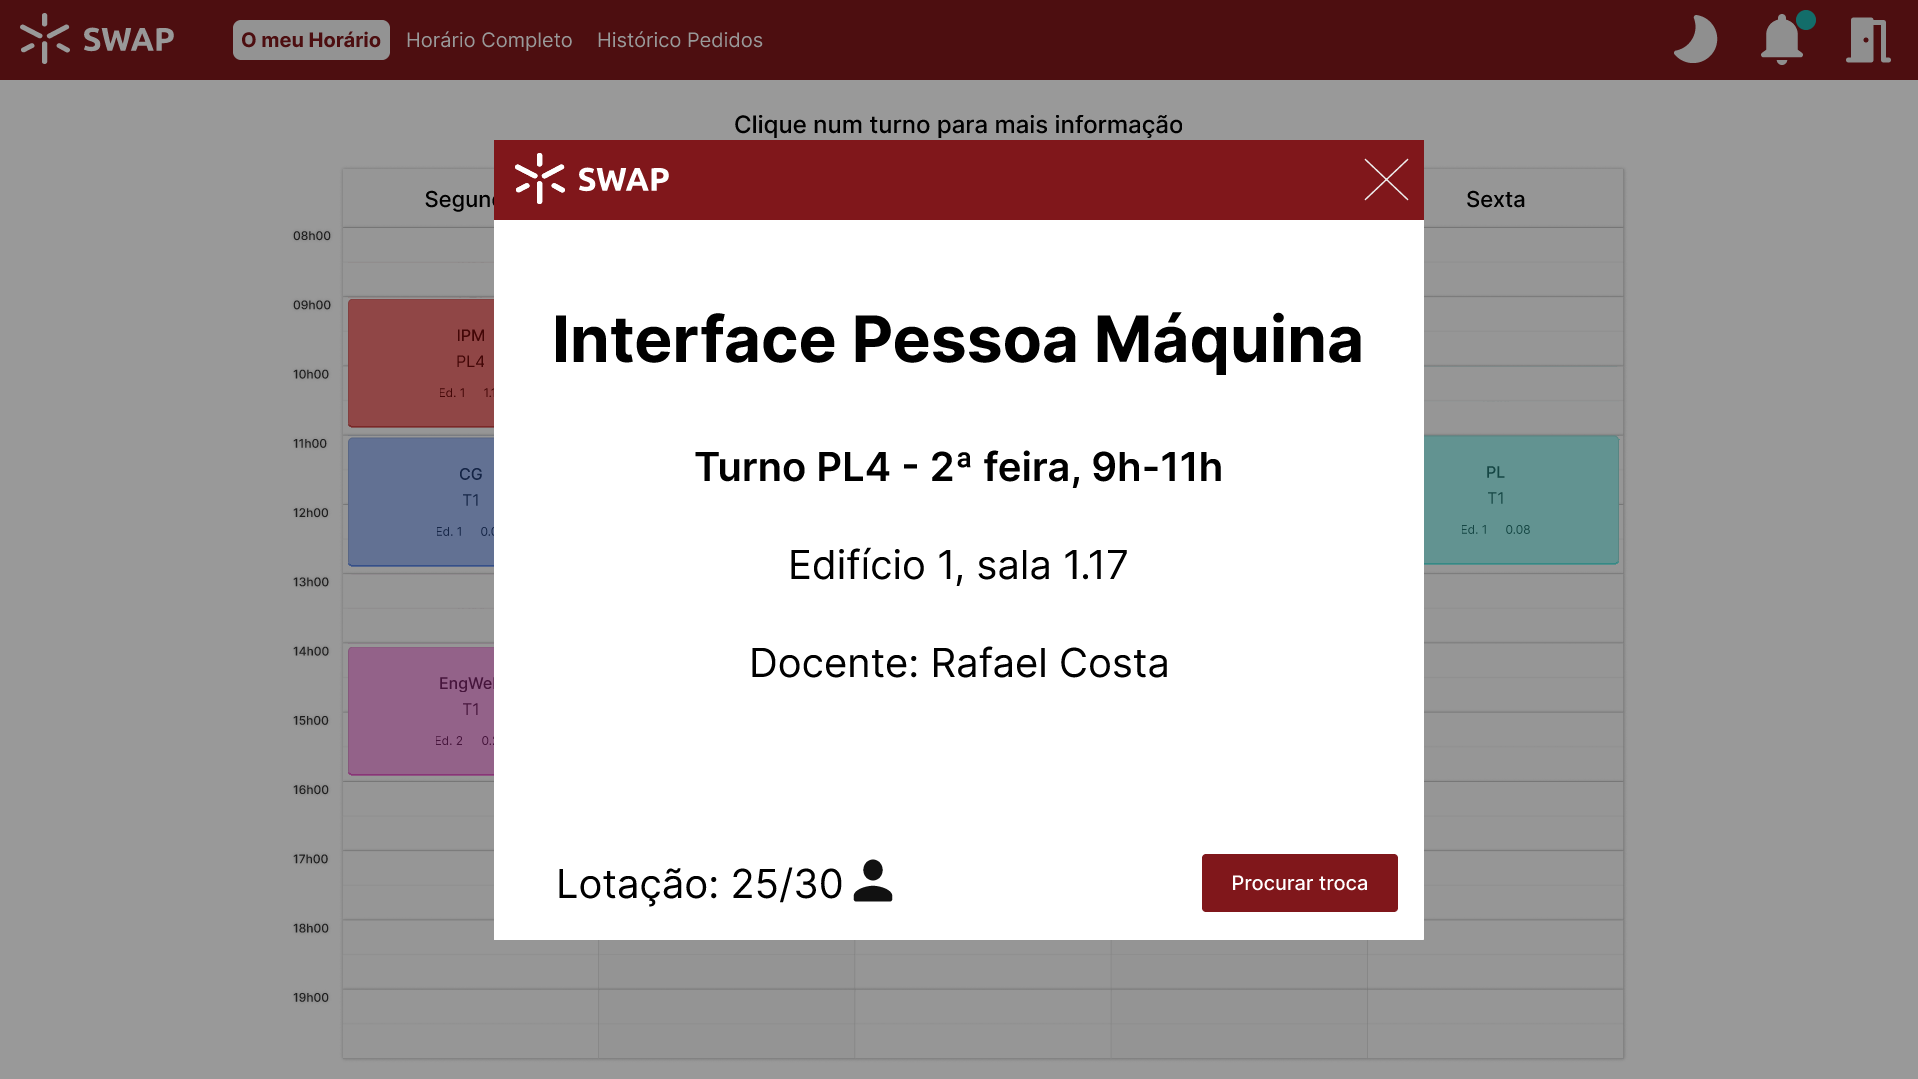
\includegraphics[width=0.6\textwidth]{res/prototype/dialogo-informacao-turno.png}
    \caption{Captura de ecrã do diálogo com informação de um turno na página ``O meu Horário''.}
    \label{dialogo-informacao-turno}
\end{figure}

A partir deste diálogo, como referido no cenário 4, é possível que o utilizador troque o turno que
selecionou, carregando no botão ``Procurar troca''. Fazê-lo deve fechar o diálogo e alterar os
conteúdos da página ``O meu Horário'' para algo como o seguinte:

\begin{figure}[H]
    \centering
    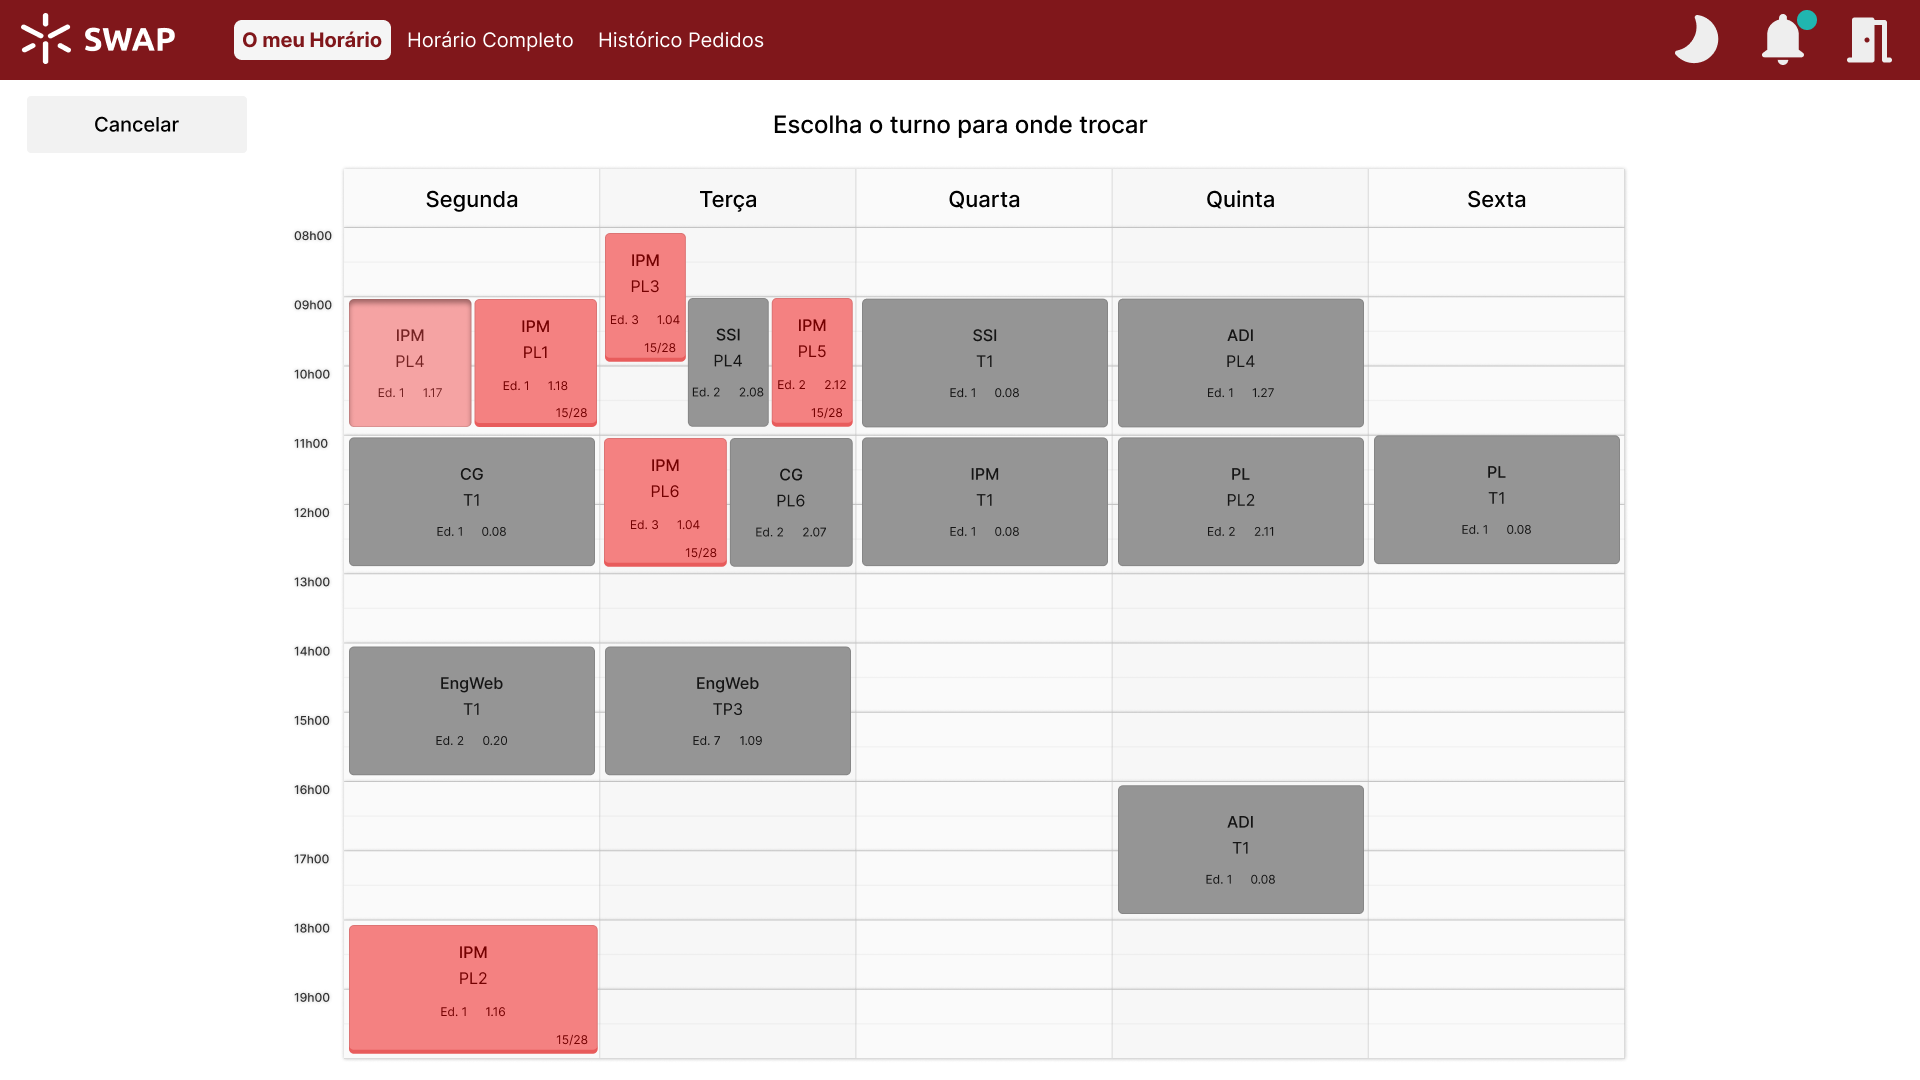
\includegraphics[width=0.8\textwidth]{res/prototype/o-meu-horario-trocar.png}
    \caption{Captura de ecrã do protótipo da página ``O meu Horário'' durante uma troca de turnos.}
    \label{o-meu-horario-trocar}
\end{figure}

Como se pode observar, os turnos em que o aluno se encontra inscrito são representados a cinzento.
Ademais, não são alterados de qualquer modo quando o cursor os sobrevoa, indicando que não é
possível interagir com eles. Por outro lado, o conjunto de turnos do mesmo tipo que o turno
selecionado (por exemplo, turnos práticos de IPM), são representados a uma cor viva, que,
juntamente com o efeito descrito na figura \ref{turno-hover}, indica que é possível interagir com
eles. Uma exceção é o turno que o utilizador pretende trocar, que é apresentado num tom entre o
cinzento e a cor viva dos restantes turnos, e sem o efeito de \emph{hover}. Deste modo, mostra-se
que não é possível trocar para este turno, mas que este turno pertence ao conjunto dos turnos
selecionados. Novamente, como o efeito de \emph{hover} não será visível para utilizadores da
aplicação com ecrãs táteis, um texto de ajuda, ``Escolha o turno para onde trocar'', é apresentado
no topo da página.

Nesta vista da página, os turnos selecionáveis pelo utilizador já apresentam a sua lotação, pois
esta informação pode ser útil para o aluno escolher para que turno deve pedir para trocar. No
entanto, é de notar que o sistema não deve impedir que um aluno envie um pedido de troca para um
turno cheio. A título de exemplo, o aluno pode ser um trabalhador estudante e o diretor de curso
colocá-lo nesse turno mesmo assim (cenário 3), ou outro aluno pode já ter enviado um pedido a
requisitar para sair desse turno. Ademais, esta interface permite facilmente ver quais as trocas de
turnos que conduzem a sobreposições, para o aluno as poder evitar. Novamente, o sistema não deve
impedir estes pedidos de troca: isso é responsabilidade do diretor de curso caso assim o deseje.

Quando o utilizador inicia o processo de troca de turno, pode aperceber-se que nenhuma opção lhe é
conveniente. Nesse caso, pode cancelar a operação carregando no botão ``Cancelar'' do lado esquerdo
da página, ou carregando na página ``O meu Horário'' na barra de navegação, reiniciando o estado
desta página e abortando a troca de turnos.

Quando se clica num turno, deve ser enviado um pedido de troca ao diretor de curso. No entanto,
como não é possível retroceder no envio deste pedido, um diálogo de confirmação deve surgir após
clicar num turno, como pode ser visto abaixo. Teve-se o cuidado de utilizar mensagens de
confirmação apenas quando estritamente necessário, ou seja, quando as ações a executar não eram
reversíveis (princípio do esforço proporcional, associado ao princípio da recuperabilidade).

\begin{figure}[H]
    \centering
    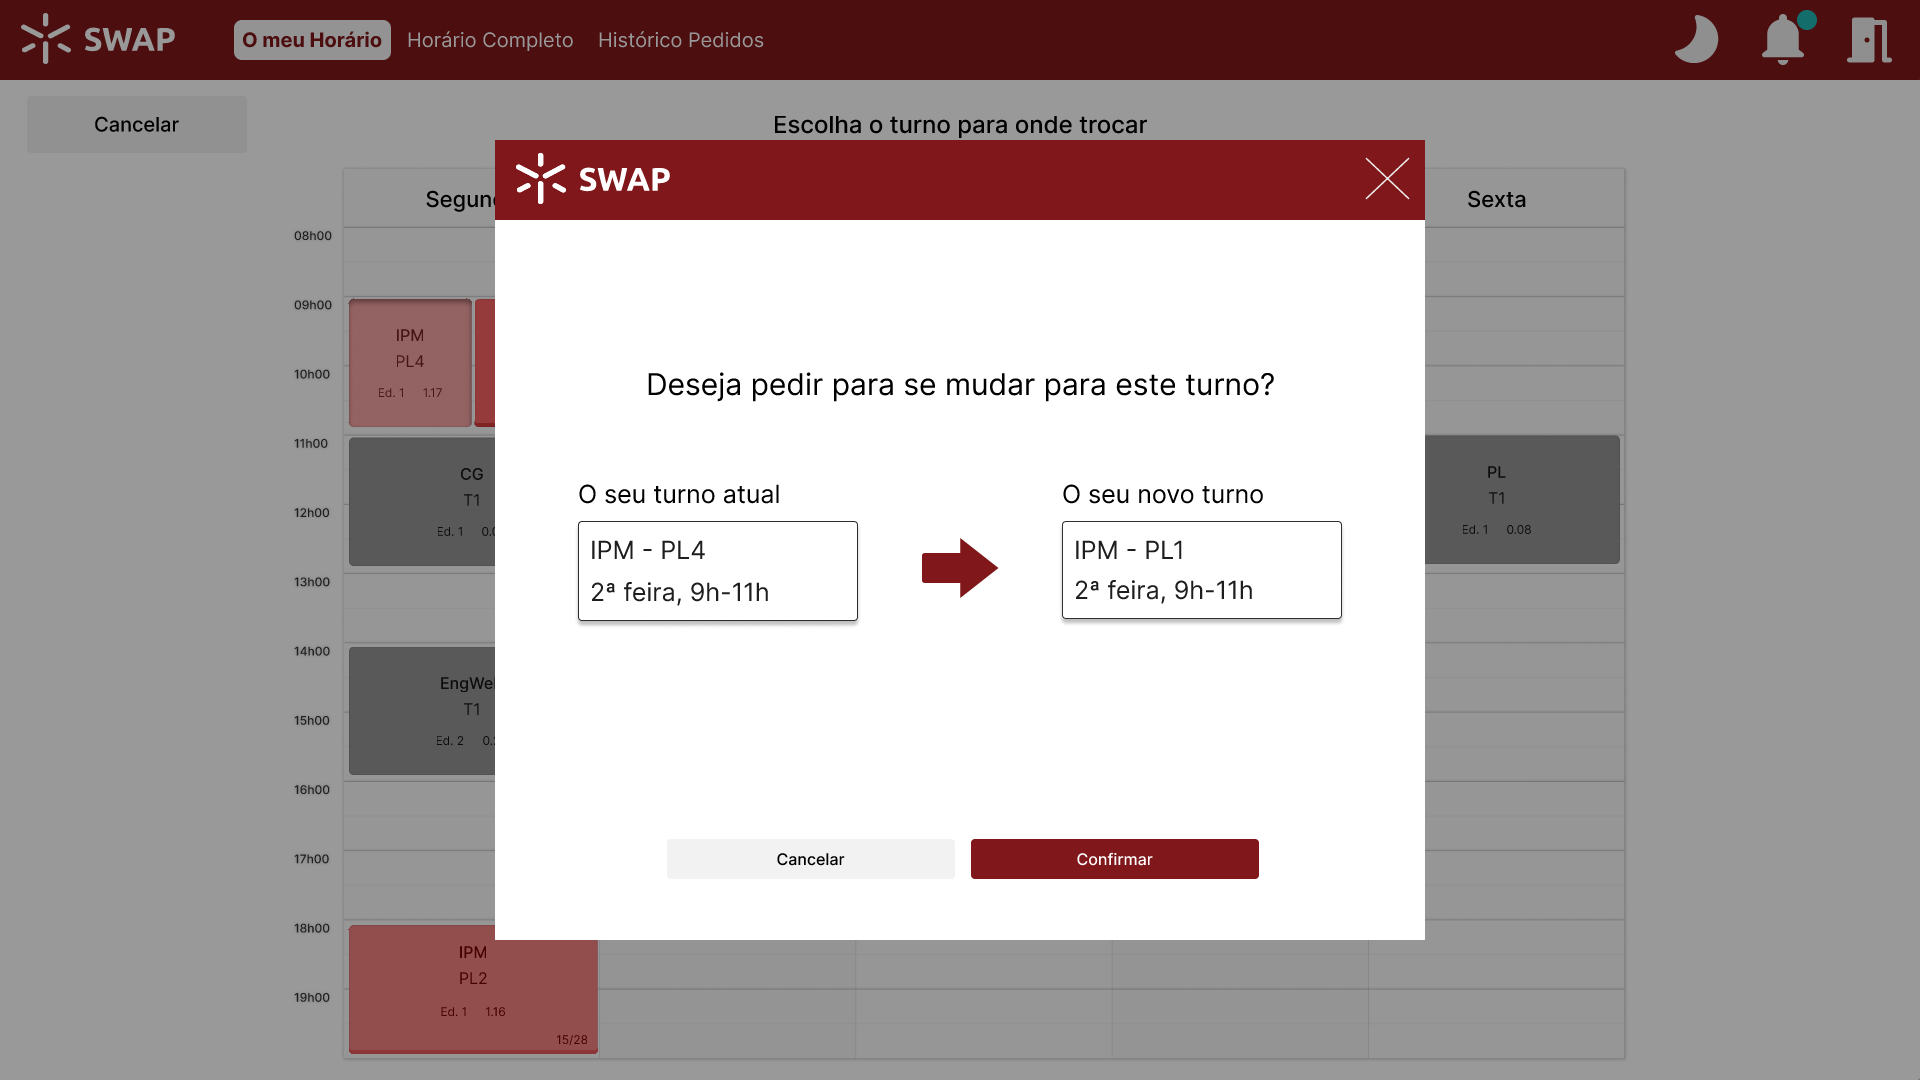
\includegraphics[width=0.8\textwidth]{res/prototype/dialogo-confirmacao-troca.png}
    \caption{
        \onehalfspacing
        Captura de ecrã do diálogo para confirmação da troca de um turno na página
        ``O meu Horário''.
    }
    \label{dialogo-confirmacao-troca}
\end{figure}

Caso o utilizador cancele a troca ou feche este diálogo, voltará à vista da página para escolha
escolha de turnos da figura \ref{o-meu-horario-trocar}. Caso confirme a troca, o utilizador será
redirecionado para o vista inicial da página ``O meu Horário'', com uma mensagem a mostrar que o
pedido de troca foi enviado. Este \emph{feedback} é especialmente importante para utilizadores menos
experientes, como os correspondentes ao perfil da Maria.

\begin{figure}[H]
    \centering
    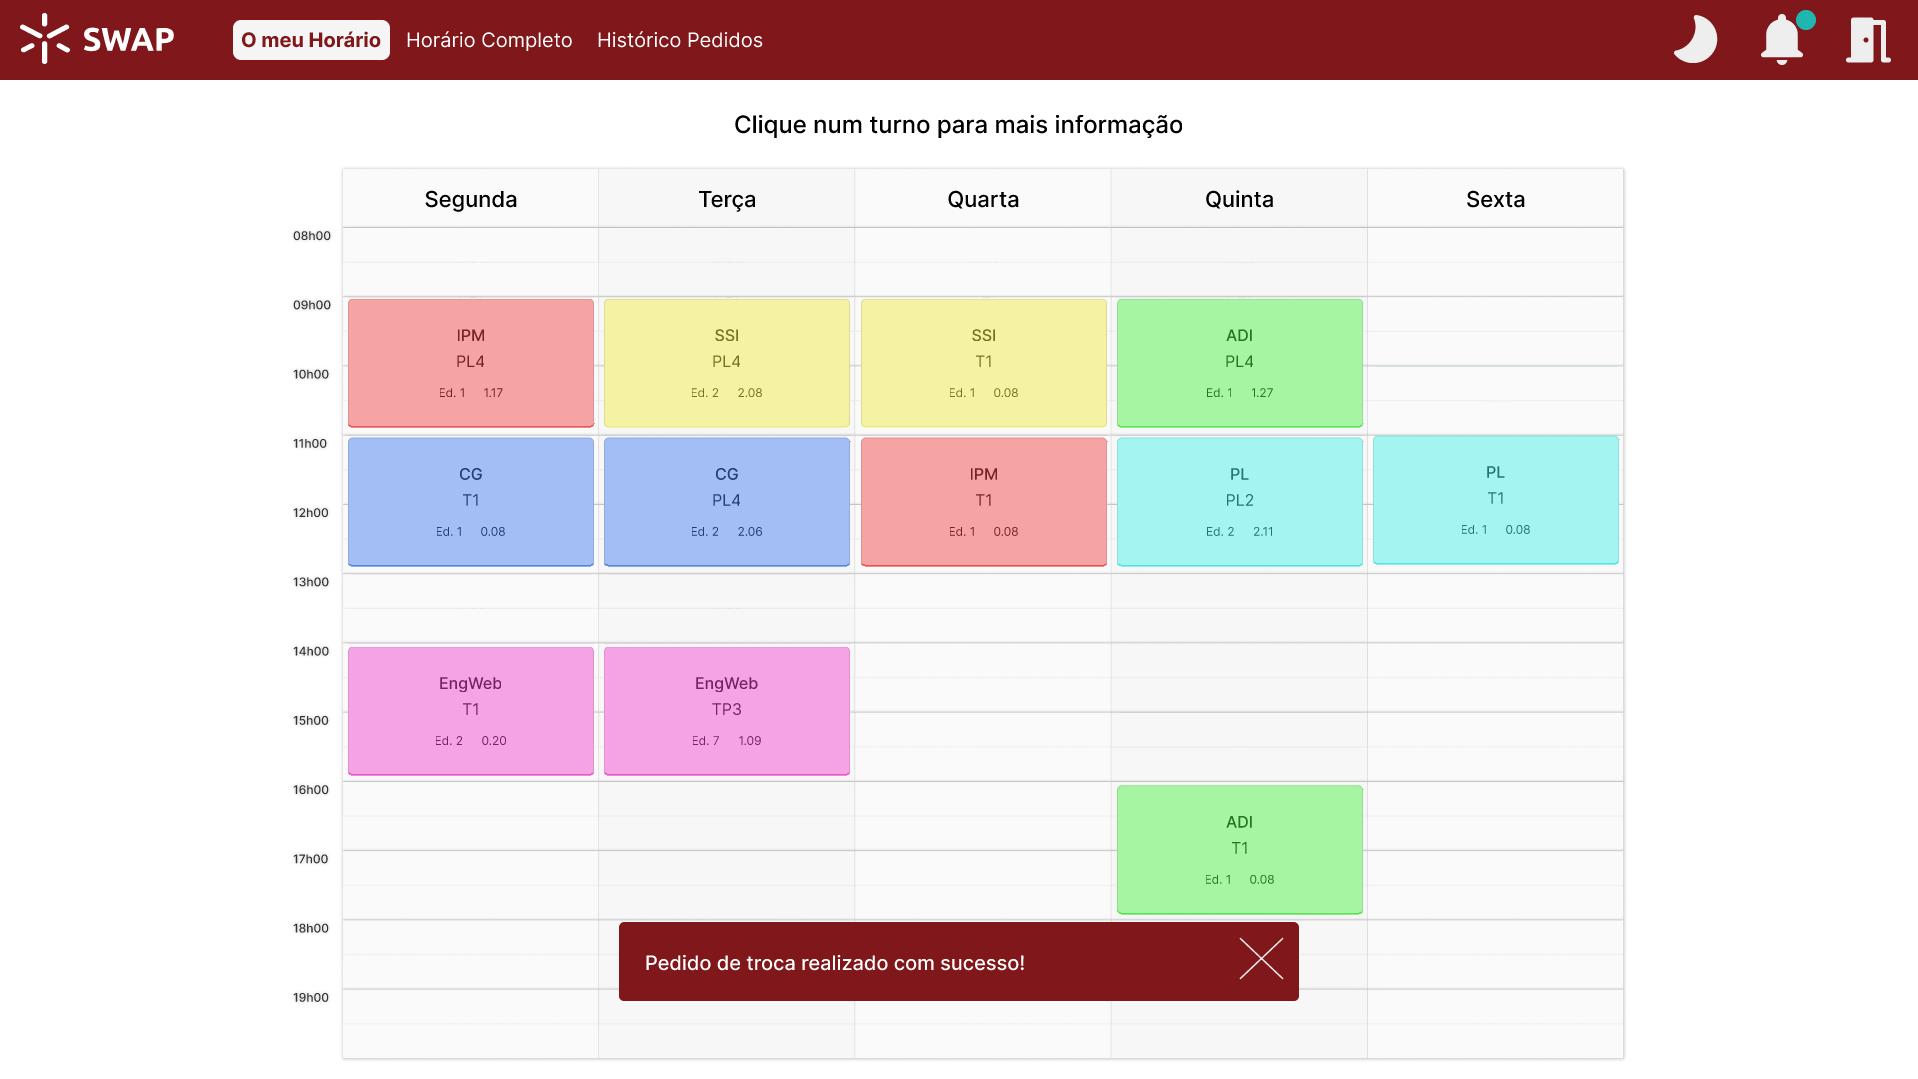
\includegraphics[width=0.8\textwidth]{res/prototype/o-meu-horario-toast-sucesso-troca.png}
    \caption{
        \onehalfspacing
        Captura de ecrã do protótipo da página ``O meu Horário'' com a confirmação de sucesso no
        envio de um pedido de troca de turno.
    }
    \label{o-meu-horario-toast-sucesso-troca}
\end{figure}

Esta mensagem deve desaparecer automaticamente após alguns segundos. No entanto, devido a limitações
do Figma, não foi possível incluir esta funcionalidade no protótipo.

\subsection{Página ``Horário Completo''}

A página ``O meu Horário'' é útil para alunos que procuram trocar apenas um turno: podem selecionar
o turno que desejam trocar, conhecer as alternativas disponíveis, e pedir para trocar para a que
mais lhes agrada. No entanto, se os alunos desejarem trocar mais do que um turno, podem querer ver
em simultâneo as várias possibilidades de troca dos vários turnos que desejam trocar. Caso a Maria
tenha mais do que uma aula na quinta de manhã, como descreve o cenário 4, poderá ter de trocar mais
do que um turno. Por este motivo, foi prototipada a página ``Horário Completo'', onde o utilizador
pode ver todos os turnos de todas as UCs em que se encontra inscrito:

\begin{figure}[H]
    \centering
    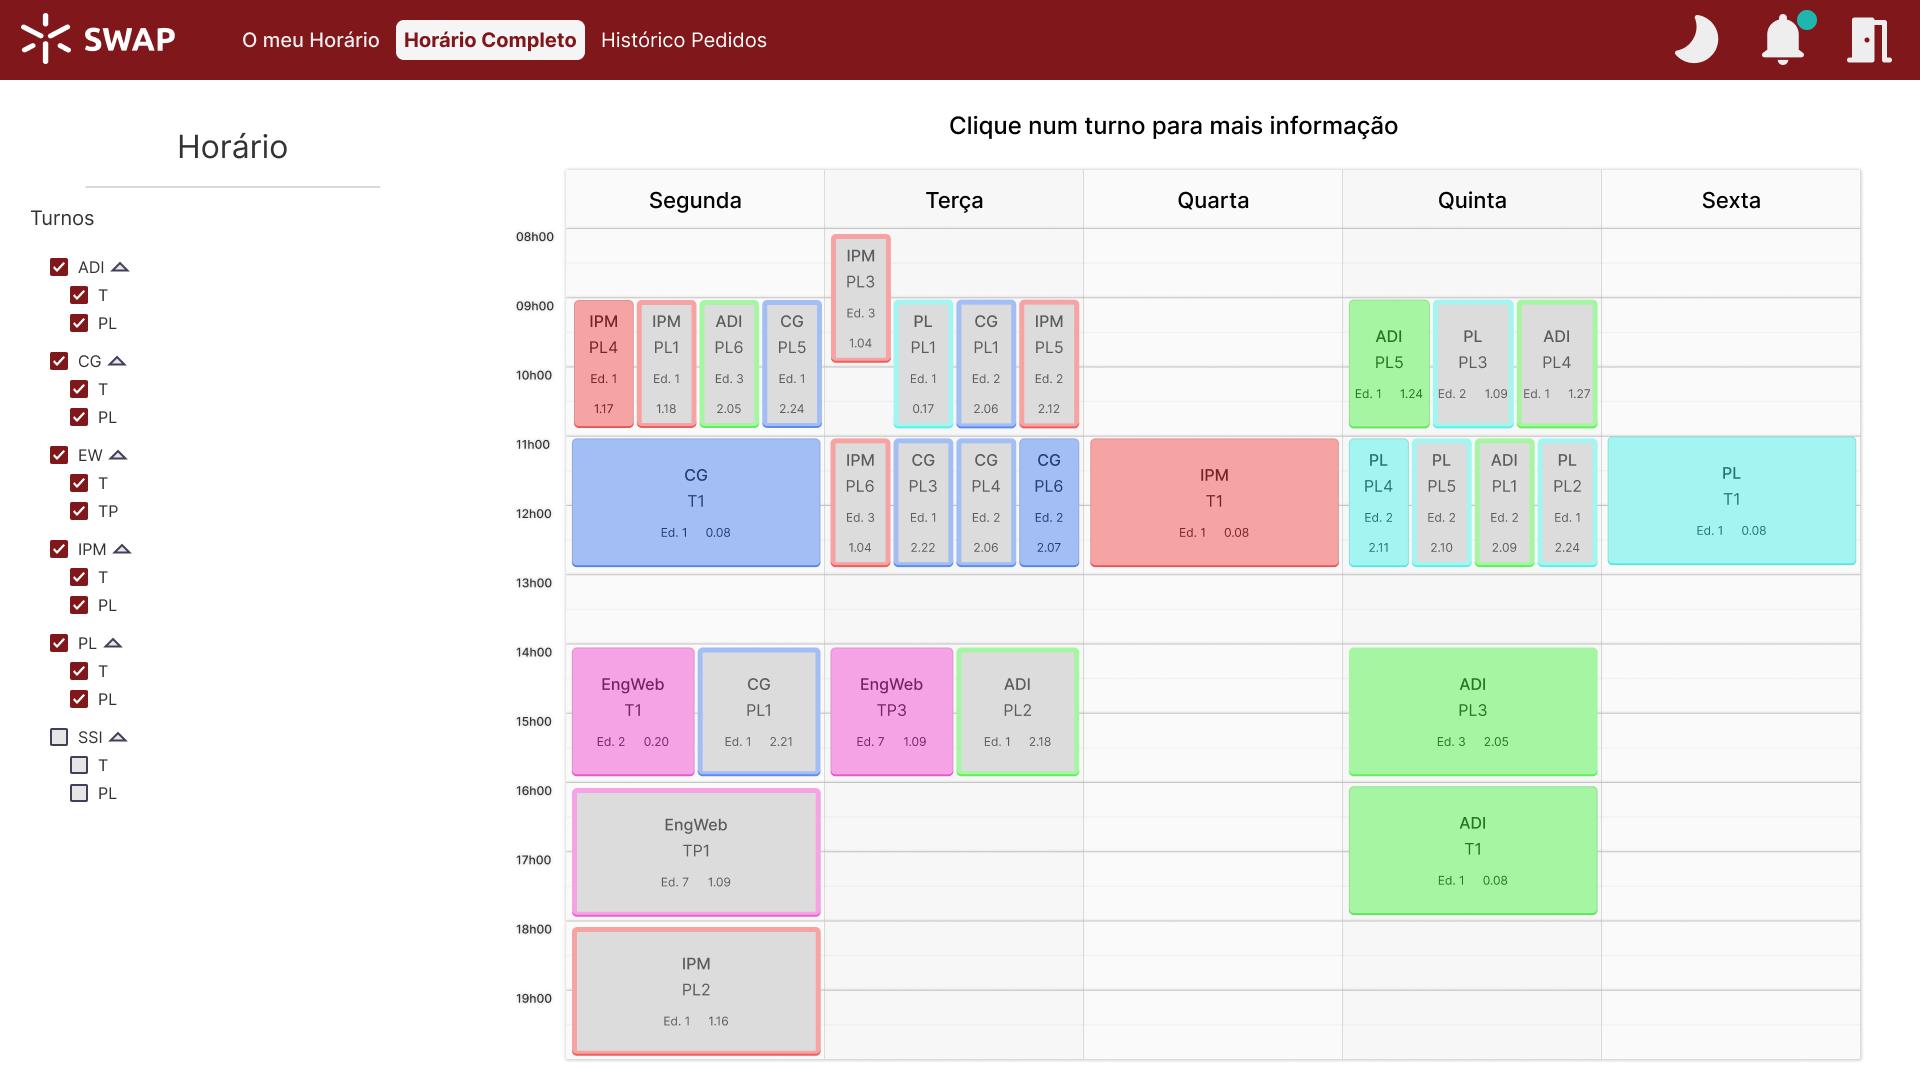
\includegraphics[width=0.8\textwidth]{res/prototype/horario-completo.png}
    \caption{Captura de ecrã do protótipo da página ``Horário Completo''.}
    \label{horario-completo}
\end{figure}

Como se pode observar, os turnos em que o aluno se encontra inscrito são apresentados em tons
coloridos, realçando as horas em que o aluno não deve escolher novos turnos, pois fazê-lo poderá
conduzir a sobreposições. Os turnos em que o aluno não se encontra inscrito são apresentados a
cinzento, com uma borda da cor correspondente à sua UC. Deste modo, o utilizador pode facilmente,
com base numa cor, identificar todos os turnos associados a uma UC.

Como podem ser muitos os turnos de todas as UCs em que o aluno se encontra inscrito, foi adicionada
uma barra lateral à página, que permite ao utilizador escolher que turnos deseja que sejam
apresentados. Deste modo, a observabilidade da página é melhorada, especialmente em ecrãs mais
pequenos. Ademais, também é adicionada alguma costumizabilidade, visto que o utilizador é capaz de
escolher que informação lhe é apresentada, podendo optar, por exemplo, por ignorar turnos de UCs
que não deseja alterar.

Caso o utilizador clique num turno para o trocar, será aberto o diálogo apresentado na figura
\ref{dialogo-informacao-turno}, a partir do qual o utilizador poderá ir para a seguinte vista da
página ``Horário Completo'':

\begin{figure}[H]
    \centering
    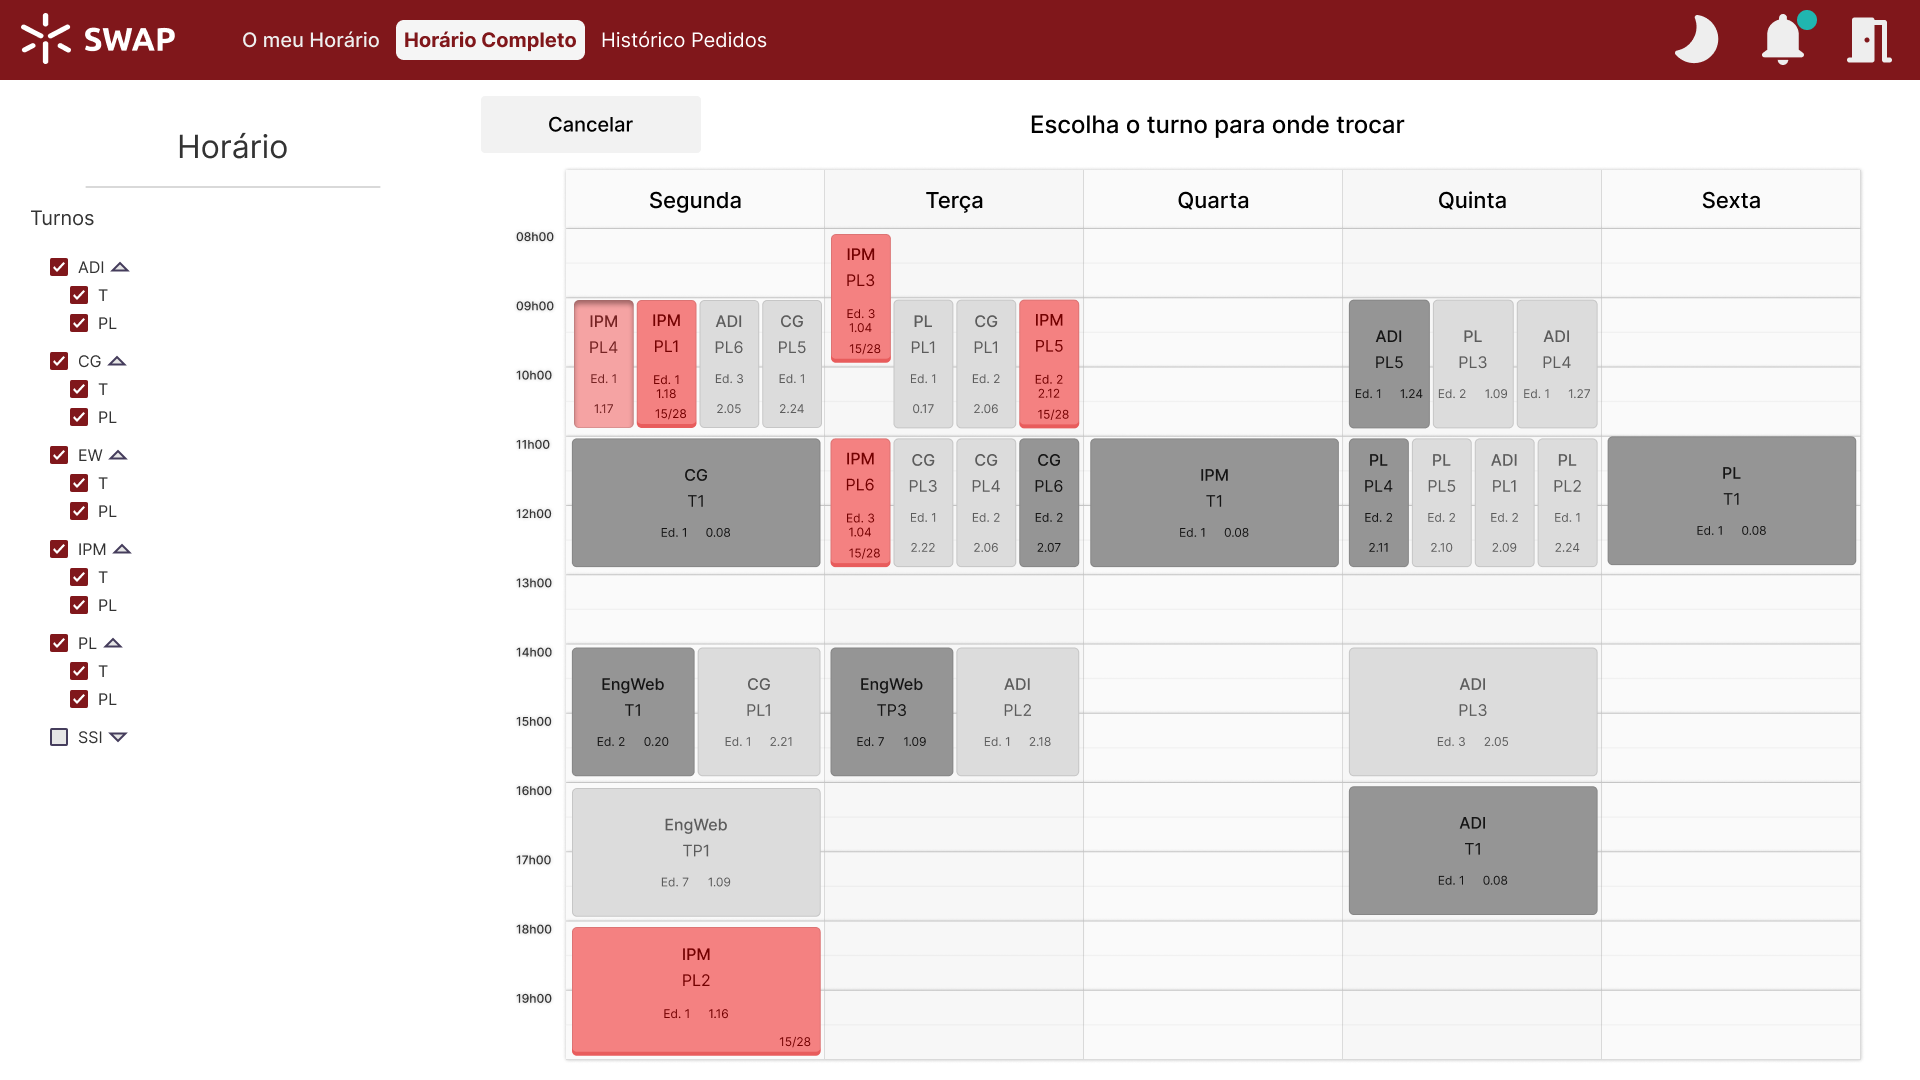
\includegraphics[width=0.8\textwidth]{res/prototype/horario-completo-trocar.png}
    \caption{
        \onehalfspacing
        Captura de ecrã do protótipo da página ``Horário Completo'' durante uma troca de turnos.
    }
    \label{horario-completo-trocar}
\end{figure}

Esta vista da página ``Horário Completo'' foi modelada com base na vista apresentada na figura
\ref{o-meu-horario-trocar}. No entanto, de uma forma consistente com a vista normal da página
``Horário Completo'', mantém-se a barra lateral, onde o utilizador pode ajustar os turnos que deseja
ver no horário. Além disso, passa a haver uma distinção entre os tons de cinzento dos turnos com os
quais não é possível interagir: um cinzento mais escuro é utilizado para apresentar os turnos nos
quais o aluno se encontra inscrito, e um cinzento mais claro é usado para apresentar os restantes
turnos. Espera-se que este realce do horário atual do aluno o ajude a detetar possíveis
sobreposições resultantes da troca de um turno.

Quando o utilizador carrega num turno, a aplicação deve comportar-se do modo previamente descrito
para a página ``O meu Horário'': o diálogo apresentado na figura \ref{dialogo-confirmacao-troca}
deve aparecer e, caso o utilizador confirme a troca de turno, o estado da página deverá ser
reiniciado, e uma confirmação de envio do pedido deverá ser apresentado:

\begin{figure}[H]
    \centering
    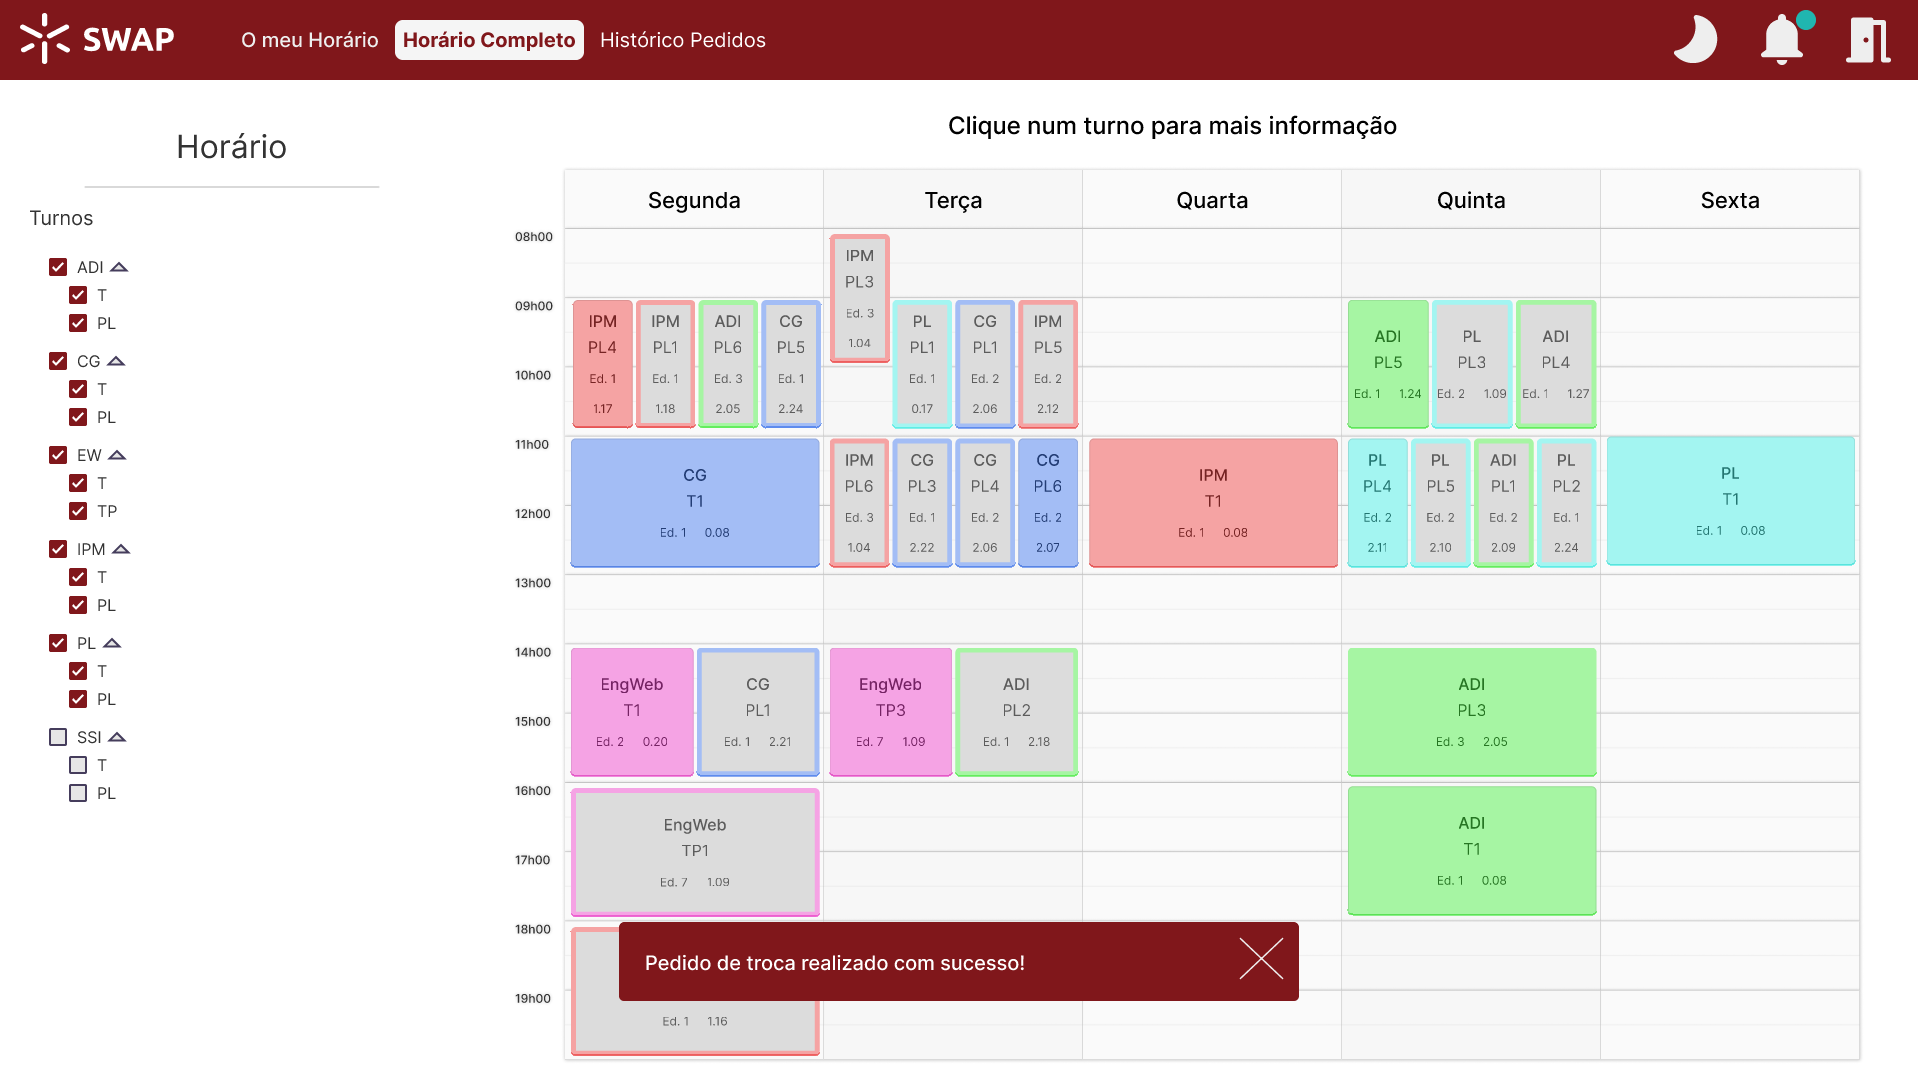
\includegraphics[width=0.8\textwidth]{res/prototype/horario-completo-toast-sucesso-troca.png}
    \caption{
        \onehalfspacing
        Captura de ecrã do protótipo da página ``Horário Completo'' com a confirmação de sucesso no
        envio de um pedido de troca de turno.
    }
    \label{horario-completo-toast-sucesso-troca}
\end{figure}

\subsection{Página ``Histórico de Pedidos''}

Foi criada uma página para apresentar ao utilizador os pedidos de troca de turnos que este fez no
passado. Esta não passa de uma lista dos pedidos, ordenados do mais recente para o mais antigo:

\begin{figure}[H]
    \centering
    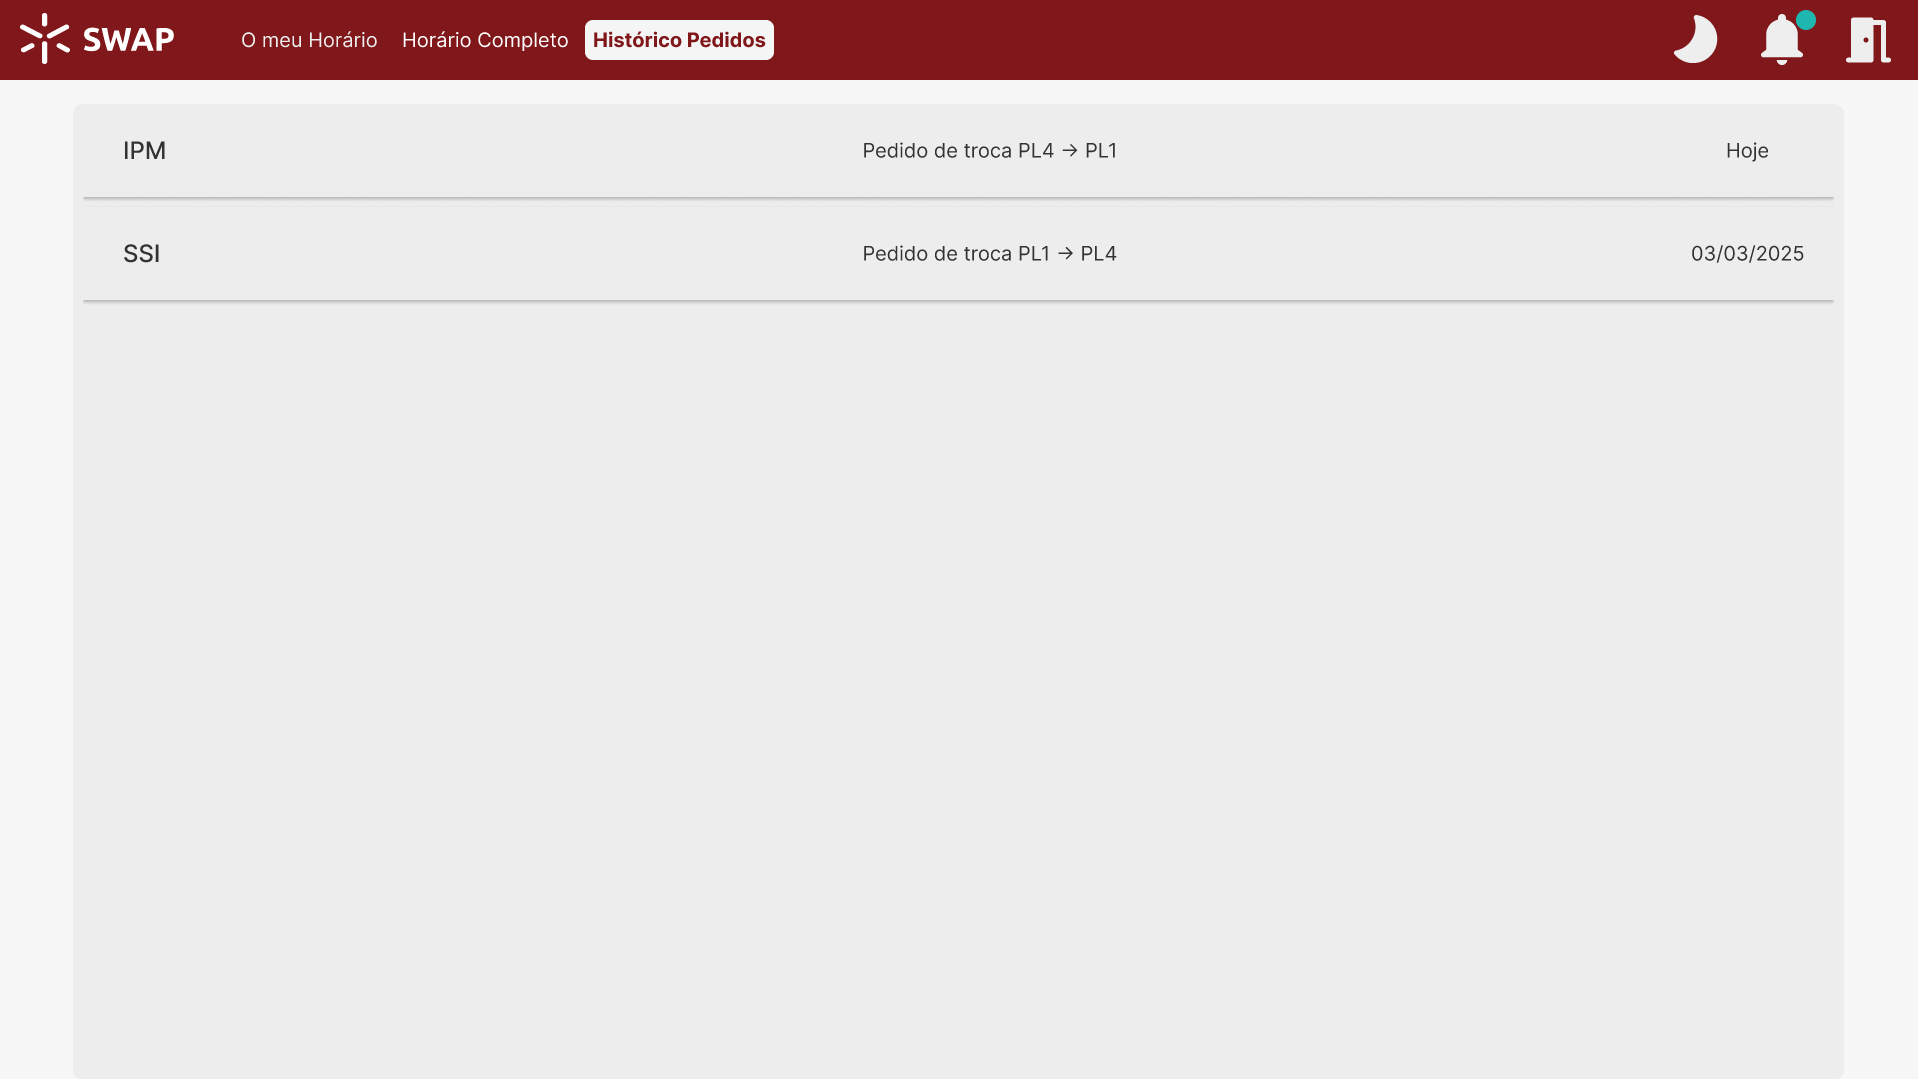
\includegraphics[width=0.8\textwidth]{res/prototype/historico-de-pedidos.png}
    \caption{Captura de ecrã do protótipo da página ``Histórico de Pedidos''.}
    \label{historico-de-pedidos}
\end{figure}

\subsection{Página ``Notificações do Aluno''}

Os alunos que utilizam a aplicação devem ter uma forma de serem notificados de eventos importantes.
Estas notificações podem ser consultadas na página cujo protótipo se apresenta abaixo, acessível
através do ícone com um sino na barra de navegação:

\begin{figure}[H]
    \centering
    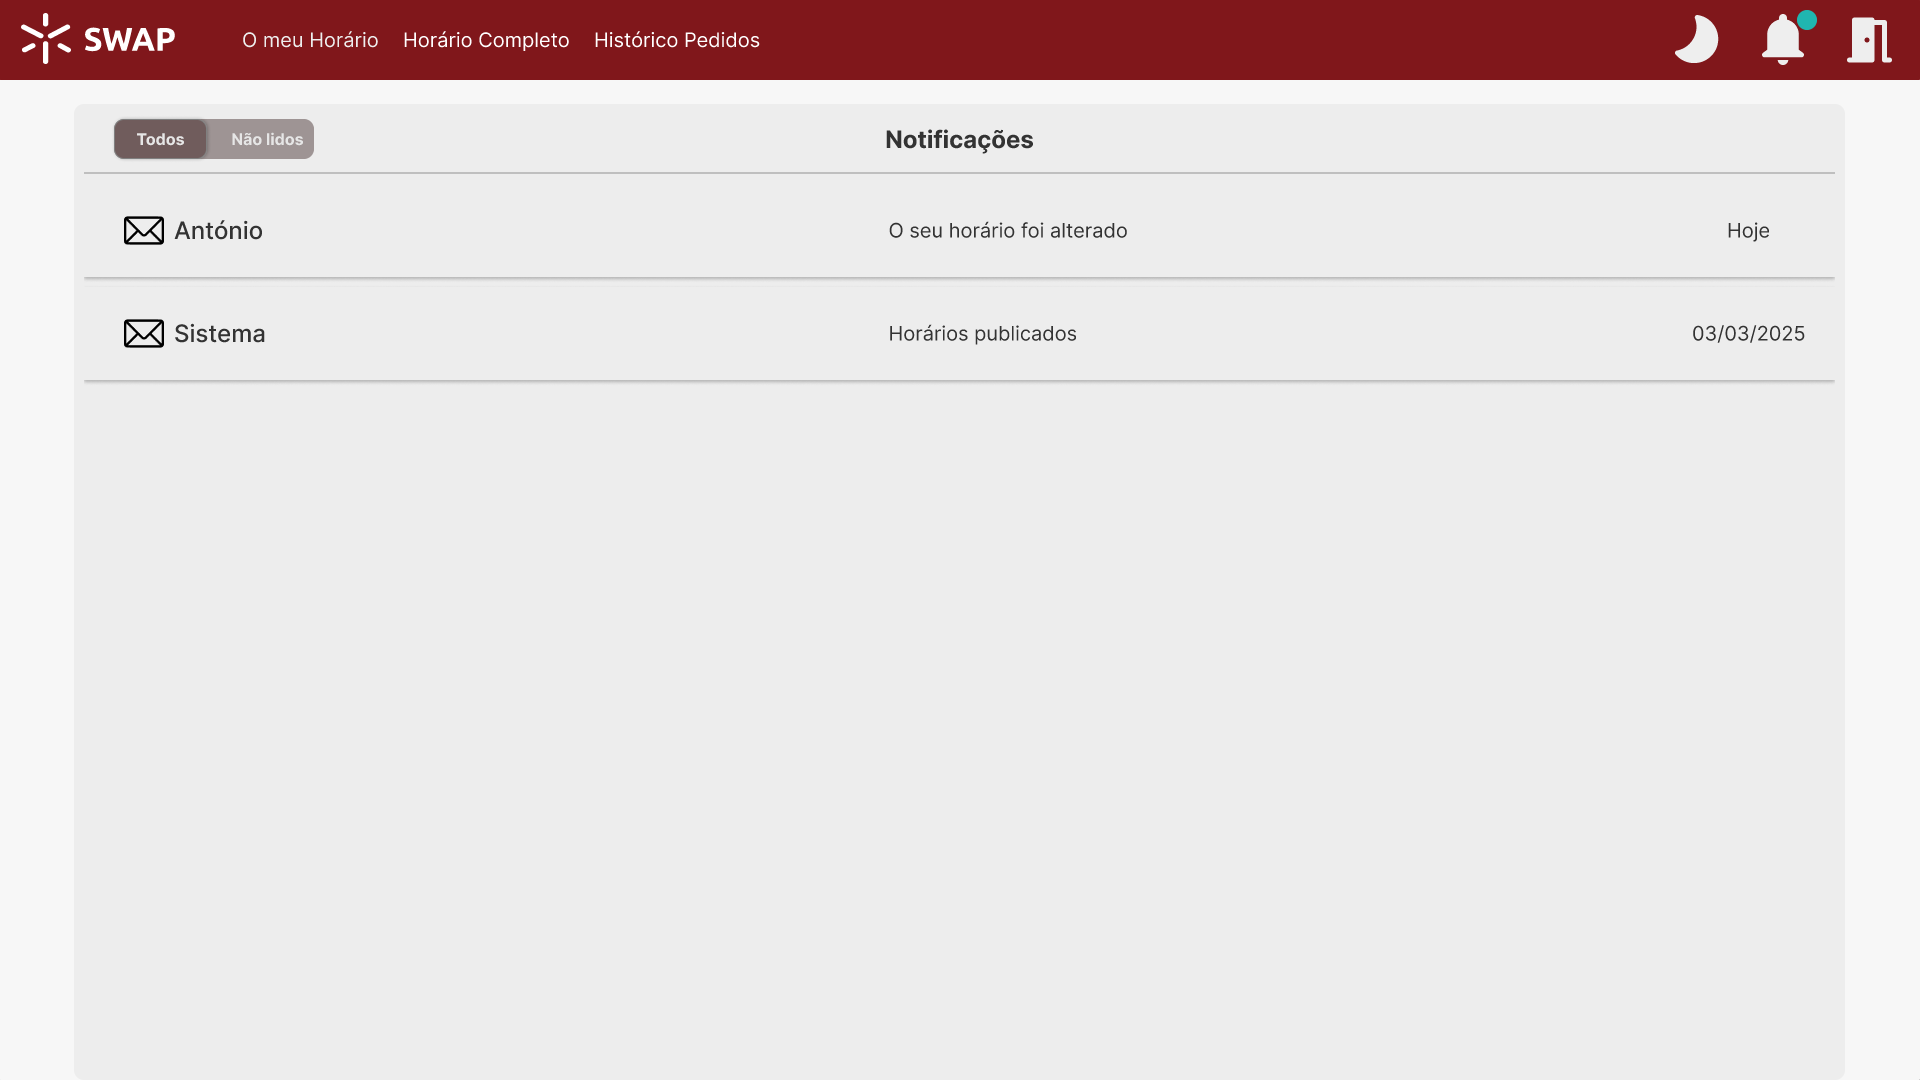
\includegraphics[width=0.8\textwidth]{res/prototype/notificacoes-aluno.png}
    \caption{Captura de ecrã do protótipo da página ``Notificações do Aluno''.}
    \label{notificacoes-aluno}
\end{figure}

Como se pode observar, esta página apresenta as notificações da mais recente para a mais antiga.
Adicionalmente, com o \emph{toggle} no canto superior esquerdo, é possível alternar entre a
apresentação de todas as notificações e apenas das notificações por ler. Ademais, como esta página
não é acessível a partir da barra de navegação, o seu título, ``Notificações'', não é realçado na
mesma, tendo de ser incluído nos seus conteúdos.

Por último, para uma boa experiência de utilização sem distrações desnecessárias, é importante que
as notificações sejam relevantes para o utilizador. Assim, definiram-se os seguintes tipos de
notificação:

\begin{itemize}
    \item Atribuição de um horário ao aluno, consequência da primeira publicação dos horários por
        parte do diretor de curso (cenário 1);
    \item Recusa de um pedido de mudança de turno pelo diretor de curso (cenário 3). Deste modo, o
        aluno sabe que o seu pedido não será satisfeito antes do diretor de curso publicar novos
        horário, fazendo com que possivelmente possa pedir para trocar outros turnos;
    \item Atualização do horário do aluno (cenário 3), que ocorre quando o diretor de curso publica
        novos horários e o conjunto de turnos que o aluno deve frequentar é alterado. É de notar que
        estas alterações podem ser outras que não a aprovação dos pedidos do aluno: o diretor é
        capaz de alterar qualquer turno que cada aluno deve frequentar.
\end{itemize}

\subsection{Página ``Resolver Problemas''}

Quando é o diretor de curso a iniciar sessão, a página que lhe será apresentada é a seguinte:

\begin{figure}[H]
    \centering
    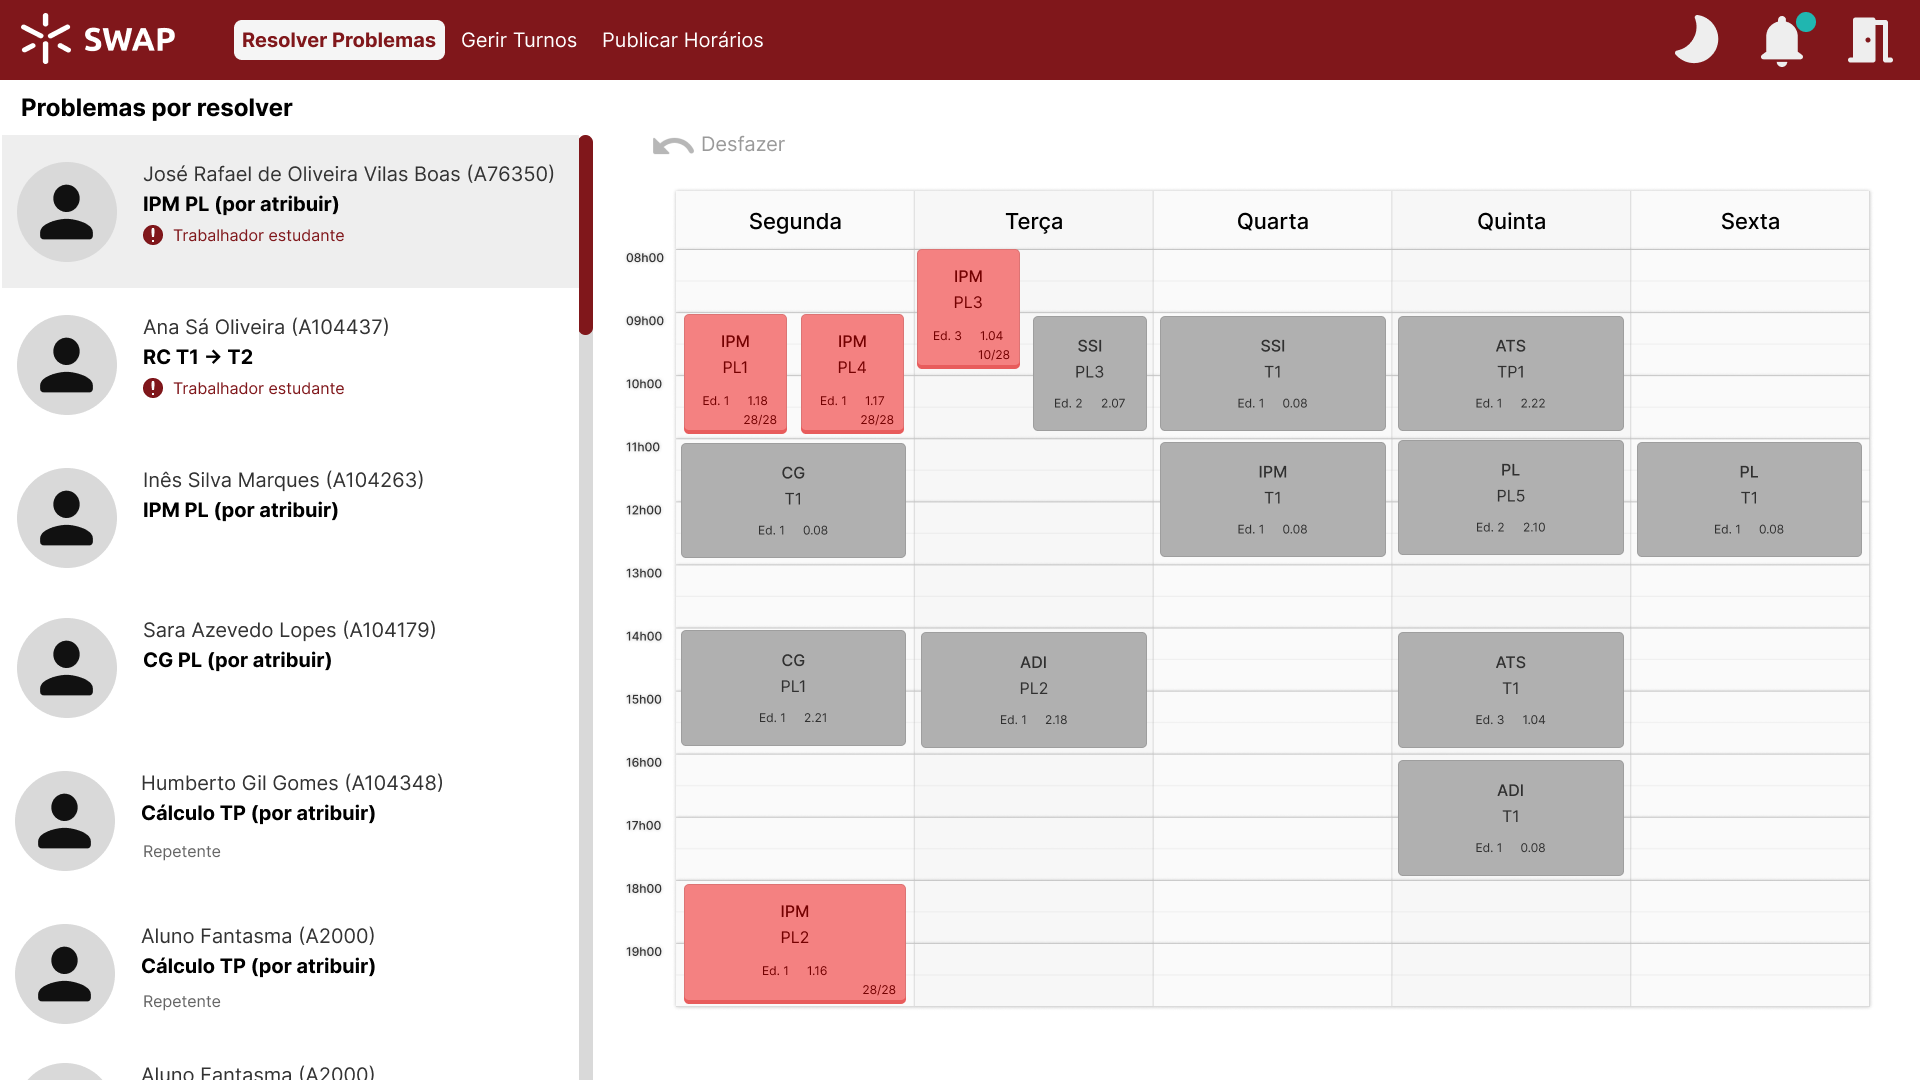
\includegraphics[width=0.8\textwidth]{res/prototype/resolver-problemas.png}
    \caption{Captura de ecrã do protótipo da página ``Resolver Problemas''.}
    \label{resolver-problemas}
\end{figure}

Como se pode observar, esta página é divida em duas colunas. Do lado esquerdo, são apresentados os
vários problemas que o diretor de curso pode resolver: alunos com turnos por atribuir (cenário 1) e
pedidos de troca de turno (cenário 3). Em primeiro lugar, devem ser apresentados os problemas
relacionados com os alunos com estatuto, e só depois os dos restantes alunos. Ademais, o segundo
critério de ordenação é o tipo de problema: primeiro são apresentados os alunos sem horário
atribuído a algumas UCs, e só depois os pedidos de troca. Assim, com esta ordem, espera-se que o
utilizador se foque, em primeiro lugar, em endereçar os problemas relacionados com os alunos com
mais limitações horárias, os estudantes com estatuo, e só depois se preocupe com os restantes,
priorizando alunos sem horário sobre preferências horárias de alunos. O aluno apresentado no ecrã é
apresentado a um tom mais escuro, tal como qualquer aluno a ser sobrevoado pelo cursor, mostrando
que é possível interagir (no caso, clicar) nestes alunos, para mudar o problema a ser apresentado:

\begin{figure}[H]
    \centering
    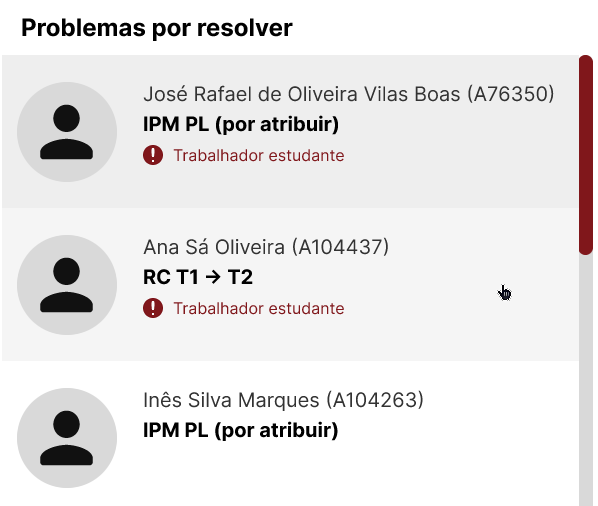
\includegraphics[width=0.5\textwidth]{res/prototype/resolver-problemas-hover.png}
    \caption{
        \onehalfspacing
        Cores de alunos escolhido para visualização, sobrevoado pelo rato, e sem alteração,
        respetivamente, na página ``Resolver Problemas''.
    }
    \label{resolver-problemas-hover}
\end{figure}

Do lado direito da página, surge o horário do aluno, a cinzento, e os turnos que lhe podem ser
atribuídos, a uma cor viva, que muda quando o cursor os sobrevoa, indicando que é possível interagir
com os mesmos. Clicar num turno abaixo da sua sua capacidade deve colocar o aluno nesse turno,
marcar o problema como resolvido, e automaticamente prosseguir para o próximo problema. No entanto,
caso o turno esteja cheio, o seguinte diálogo deve ser apresentado:

\begin{figure}[H]
    \centering
    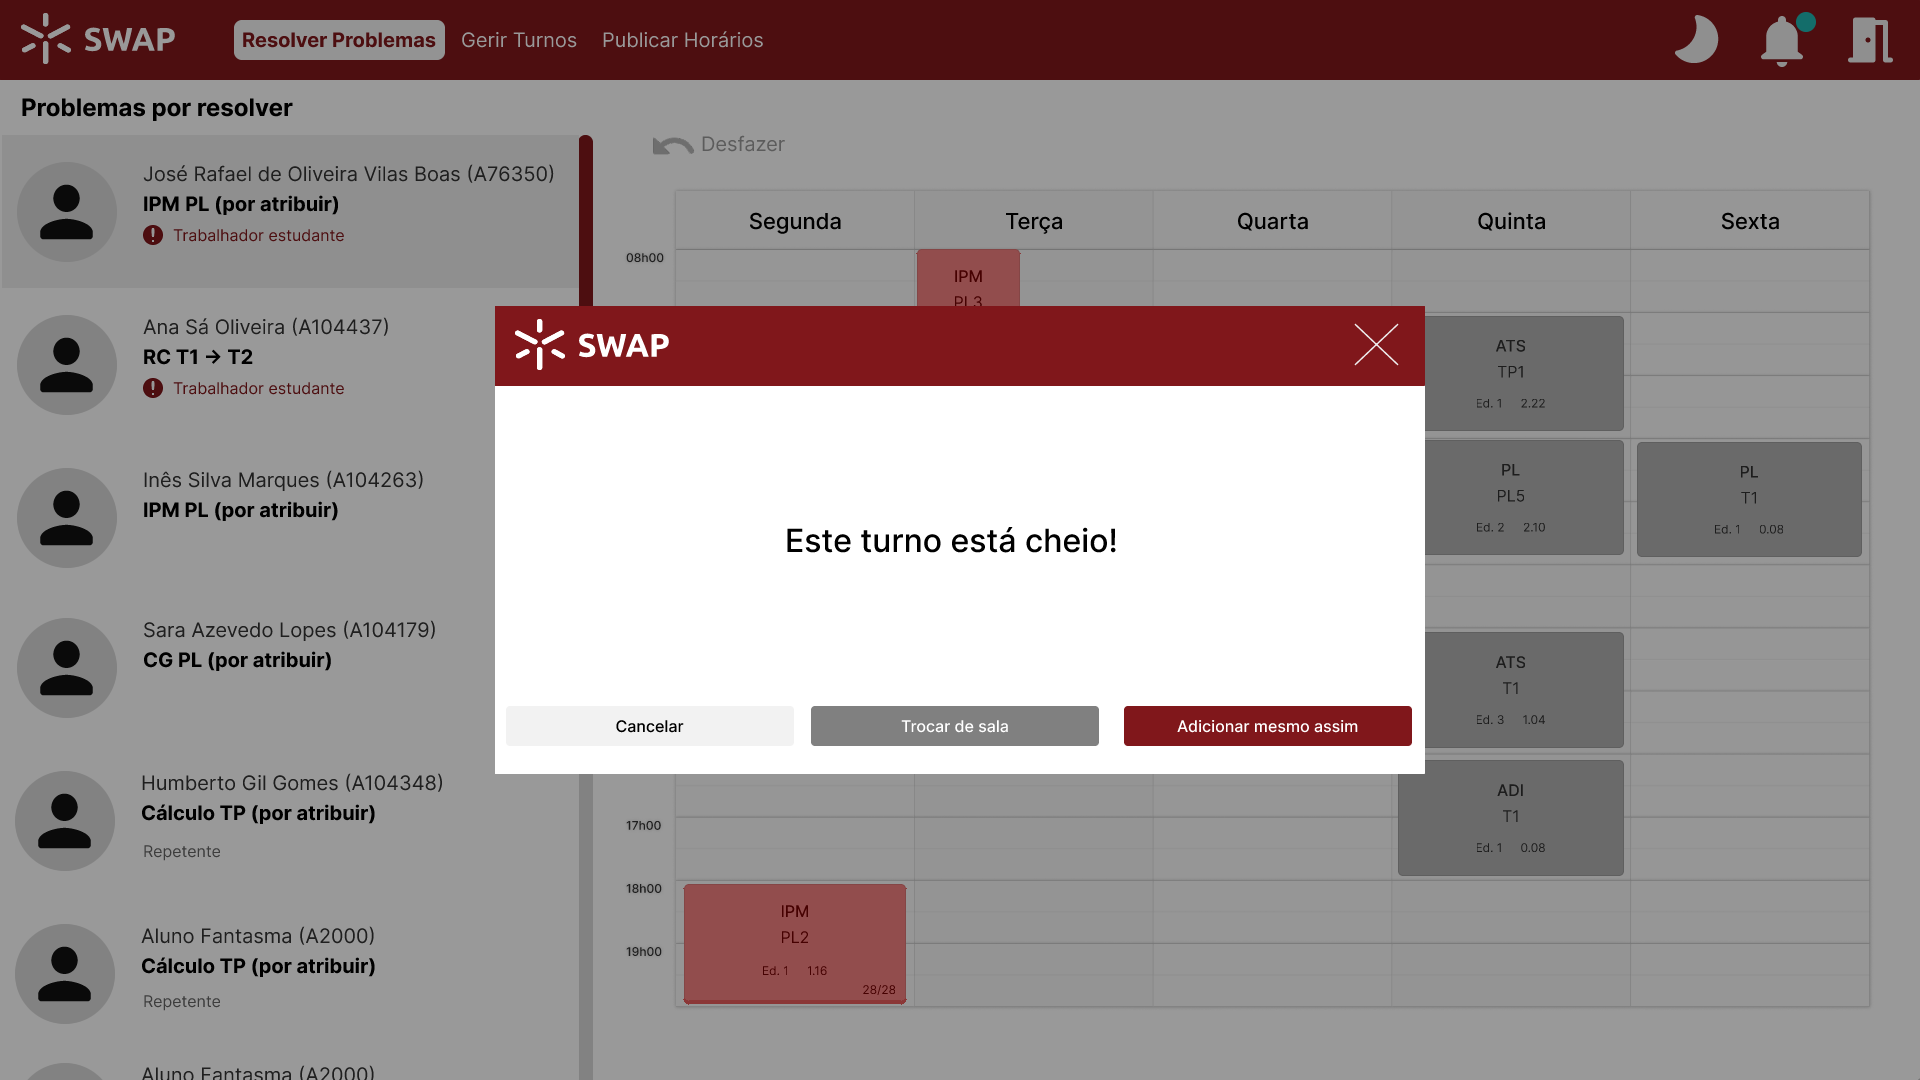
\includegraphics[width=0.8\textwidth]{res/prototype/dialogo-turno-cheio.png}
    \caption{
        \onehalfspacing
        Captura de ecrã do diálogo de adição de um aluno a um turno cheio, na página
        ``Resolver Problemas''.
    }
    \label{dialogo-turno-cheio}
\end{figure}

Este diálogo relembra o utilizador de que este se encontra a adicionar um aluno a um turno cheio,
dando-lhe a opção de cancelar essa operação, de trocar a sala do turno (cenário 3), ou de colocar o
aluno no turno e deixar que a sua lotação ultrapasse a sua capacidade (também cenário 3). É de notar
que apenas o botão para troca de sala, que redireciona o utilizador para a página ``Gerir Turno'',
não se encontra ativo para todos os turnos práticos, visto que a sua capacidade pode não ser
limitada pela capacidade da sala em que são lecionados. Nesse caso, deve haver uma \emph{tooltip}
associada ao botão com essa informação.

Quando o problema apresentado é um de troca de turnos, o esquema de cores dos turnos segue o
utilizado na página ``O meu horário'' (ver figura \ref{o-meu-horario-trocar}):

\begin{figure}[H]
    \centering
    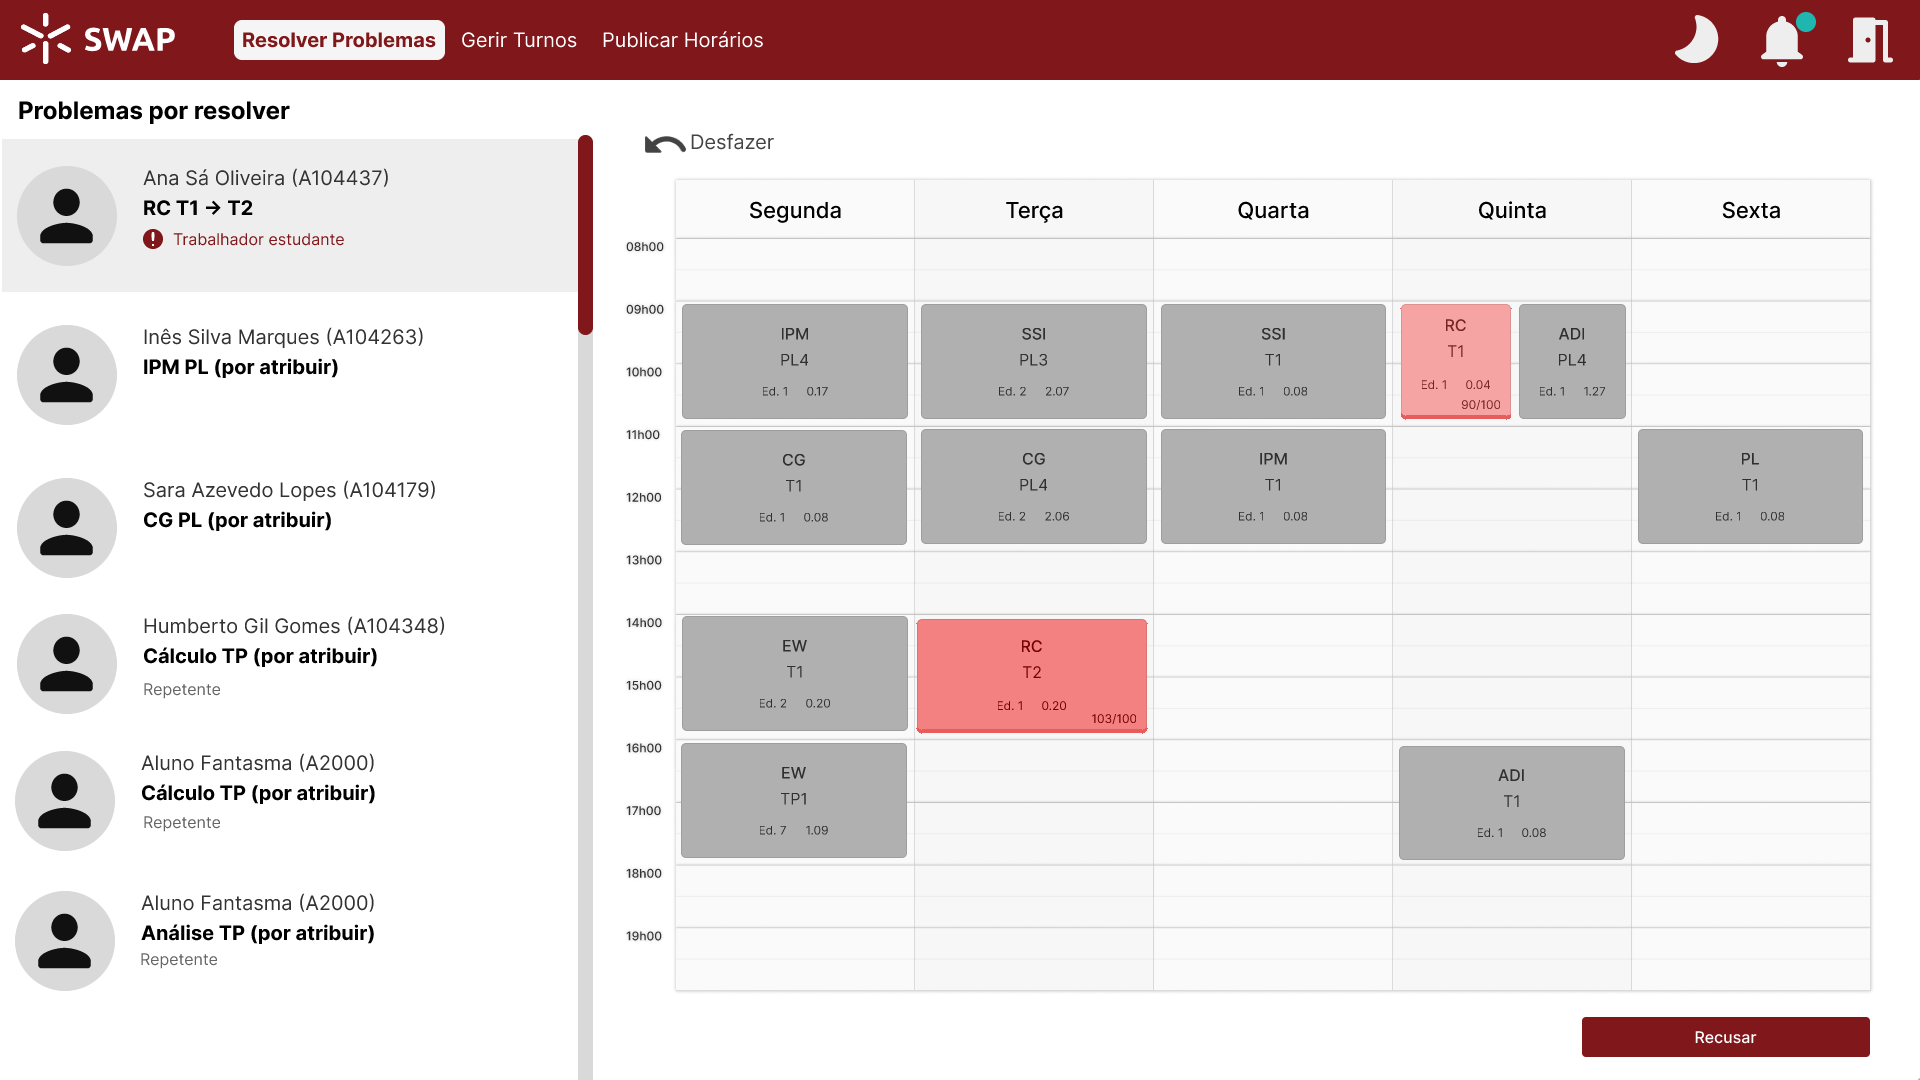
\includegraphics[width=0.8\textwidth]{res/prototype/resolver-problemas-pedido.png}
    \caption{
        \onehalfspacing
        Captura de ecrã do protótipo da página ``Resolver Problemas'' durante a resolução de um
        pedido de troca de turno.
    }
    \label{resolver-problemas-pedido}
\end{figure}

No canto superior esquerdo, pode observar-se um botão para desfazer a ação previamente realizada,
o que faz com que seja fácil recuperar de erros. No entanto, é impossível reverter a recusa de
pedidos de troca de alunos, uma vez que quando um pedido é recusado, uma notificação é enviada ao
aluno a avisá-lo. Por esse motivo, quando se recursa o pedido de um aluno usando o botão no canto
inferior diretor da página, um diálogo de confirmação surge antes, a perguntar se o utilizador tem
a certeza que deseja realizar esta ação irreversível:

\begin{figure}[H]
    \centering
    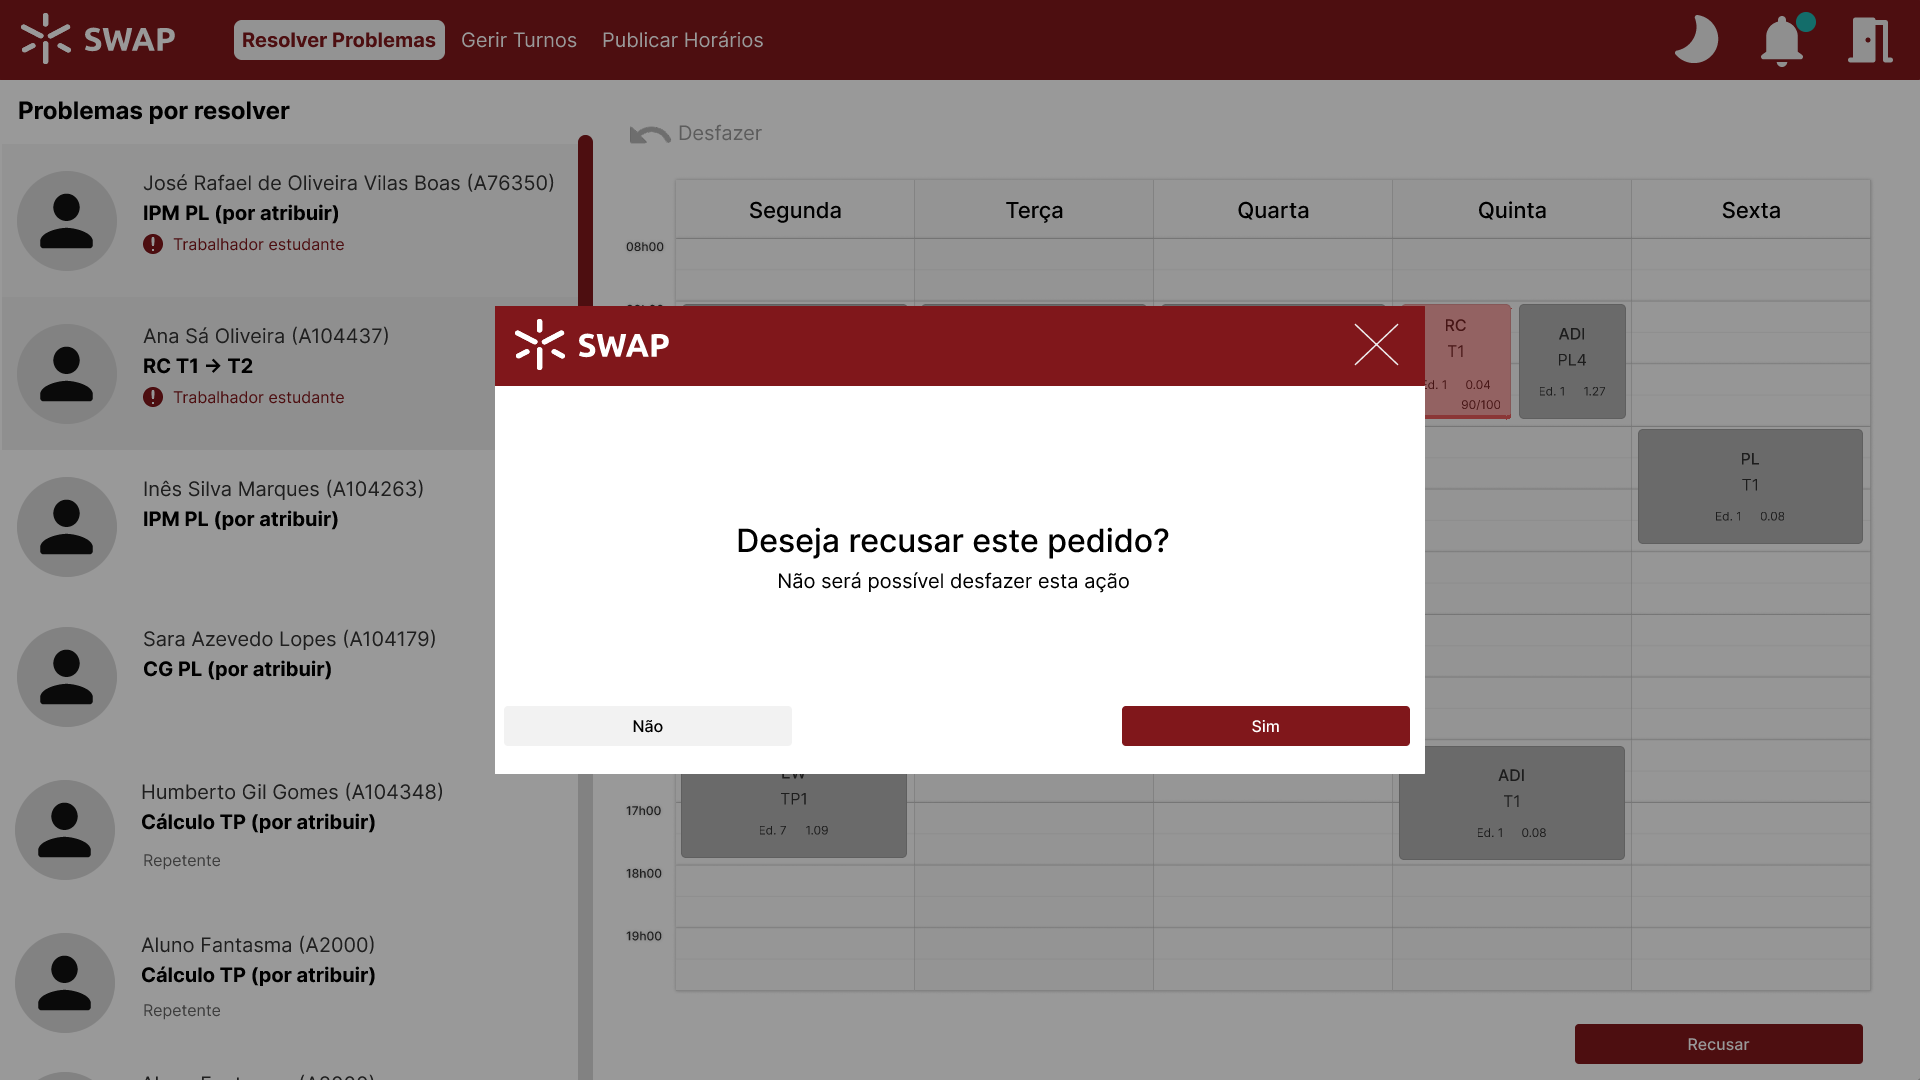
\includegraphics[width=0.8\textwidth]{res/prototype/dialogo-confirmacao-recusa.png}
    \caption{
        \onehalfspacing
        Diálogo de confirmação de recusa de um pedido de troca de turno na página
        ``Resolver Problemas''.
    }
    \label{dialogo-confirmacao-recusa}
\end{figure}

\subsection{Página ``Gerir Turnos''}

Além de resolver problemas simples de atribuição de turnos a alunos, o diretor de curso pode
precisar de fazer uma gestão mais aprofundada de cada turno, mesmo além da que é descrita pelo
cenário 3. Ações como manualmente tirar alunos de turnos para depois os colocar noutros devem ser
suportadas, para permitir que o diretor de curso faça uma otimização manual dos horários, procurando
garantir que os horários de todos os alunos são válidos e que nenhum turno excede a sua capacidade.
Para escolher um turno para gerir, o diretor de curso pode utilizar a página cujo protótipo se
apresenta abaixo:

\begin{figure}[H]
    \centering
    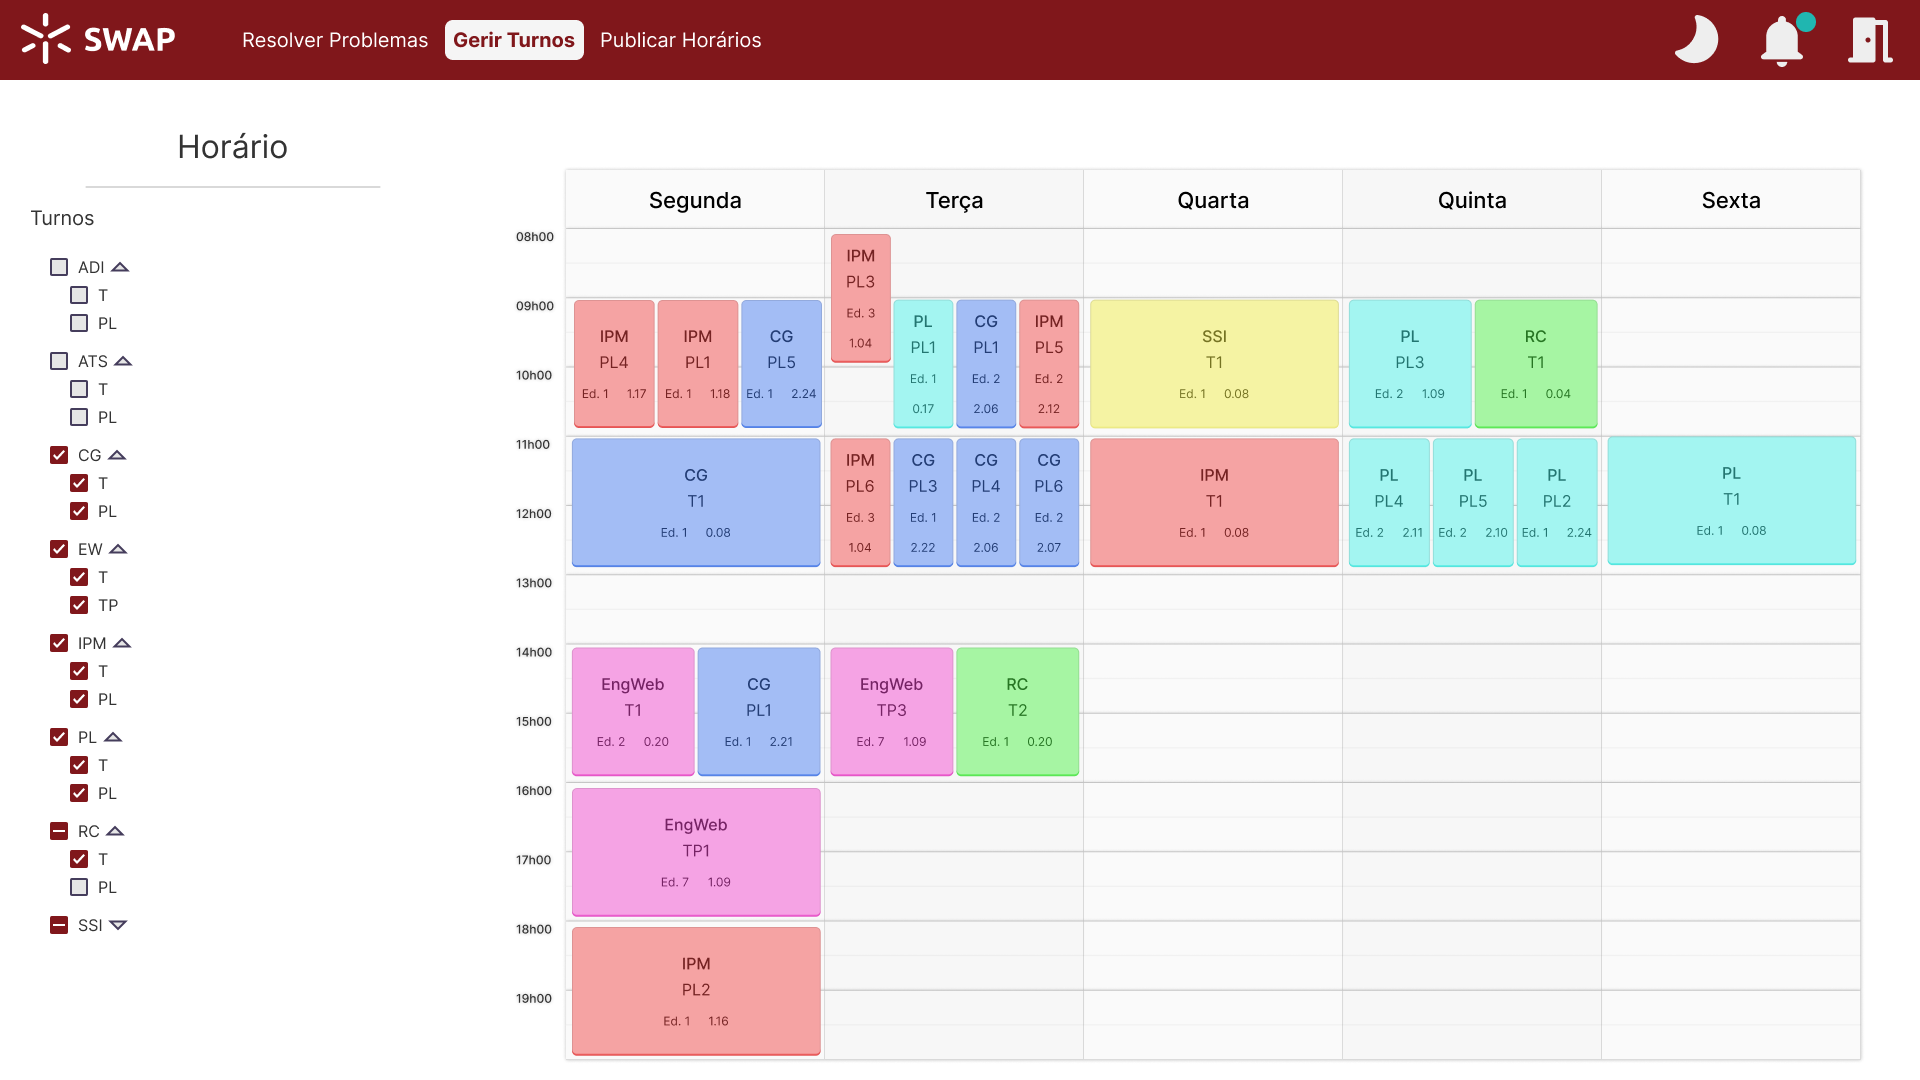
\includegraphics[width=0.8\textwidth]{res/prototype/gerir-turnos.png}
    \caption{Captura de ecrã do protótipo da página ``Gerir Turnos''.}
    \label{gerir-turnos}
\end{figure}

Esta página é semelhante à página ``Horário Completo'', onde todos os turnos de todas as UCs em que
um aluno se encontra inscrito lhe são apresentadas. Agora, sem a necessidade de realçar o horário do
aluno, todos os turnos são apresentados com a cor que identifica a sua UC. A barra lateral é ainda
mais importante: deve ser possível que o diretor de curso consulte todos os turnos de todas as UCs
do curso, e não apenas as quais um dado aluno se encontra inscrito. Isto é um grande desafio de
observabilidade, uma vez que não é possível apresentar todos os turnos em simultâneo no espaço
finito do ecrã, e deve ser dada ao diretor de curso a possibilidade de escolher quais ele pretende
visualizar. Optou-se por um sistema em que o diretor de curso escolhe que turnos deseja visualizar
com base na sua UC, e não com base numa pesquisa pelo nome do turno, visto que a gestão de um turno
pode precisar da modificação de outros turnos da mesma UC (por exemplo, para mudar um aluno de
turno). Ademais, a visualização destes turnos numa estrutura de horário permite que o diretor de
curso facilmente identifique turnos à mesma hora que outros.

\subsection{Página ``Gerir Turno''}

Quando o diretor de curso carrega num turno da página ``Gerir Turnos'', será redirecionado para a
página ``Gerir Turno'', cujo protótipo se apresenta abaixo:

\begin{figure}[H]
    \centering
    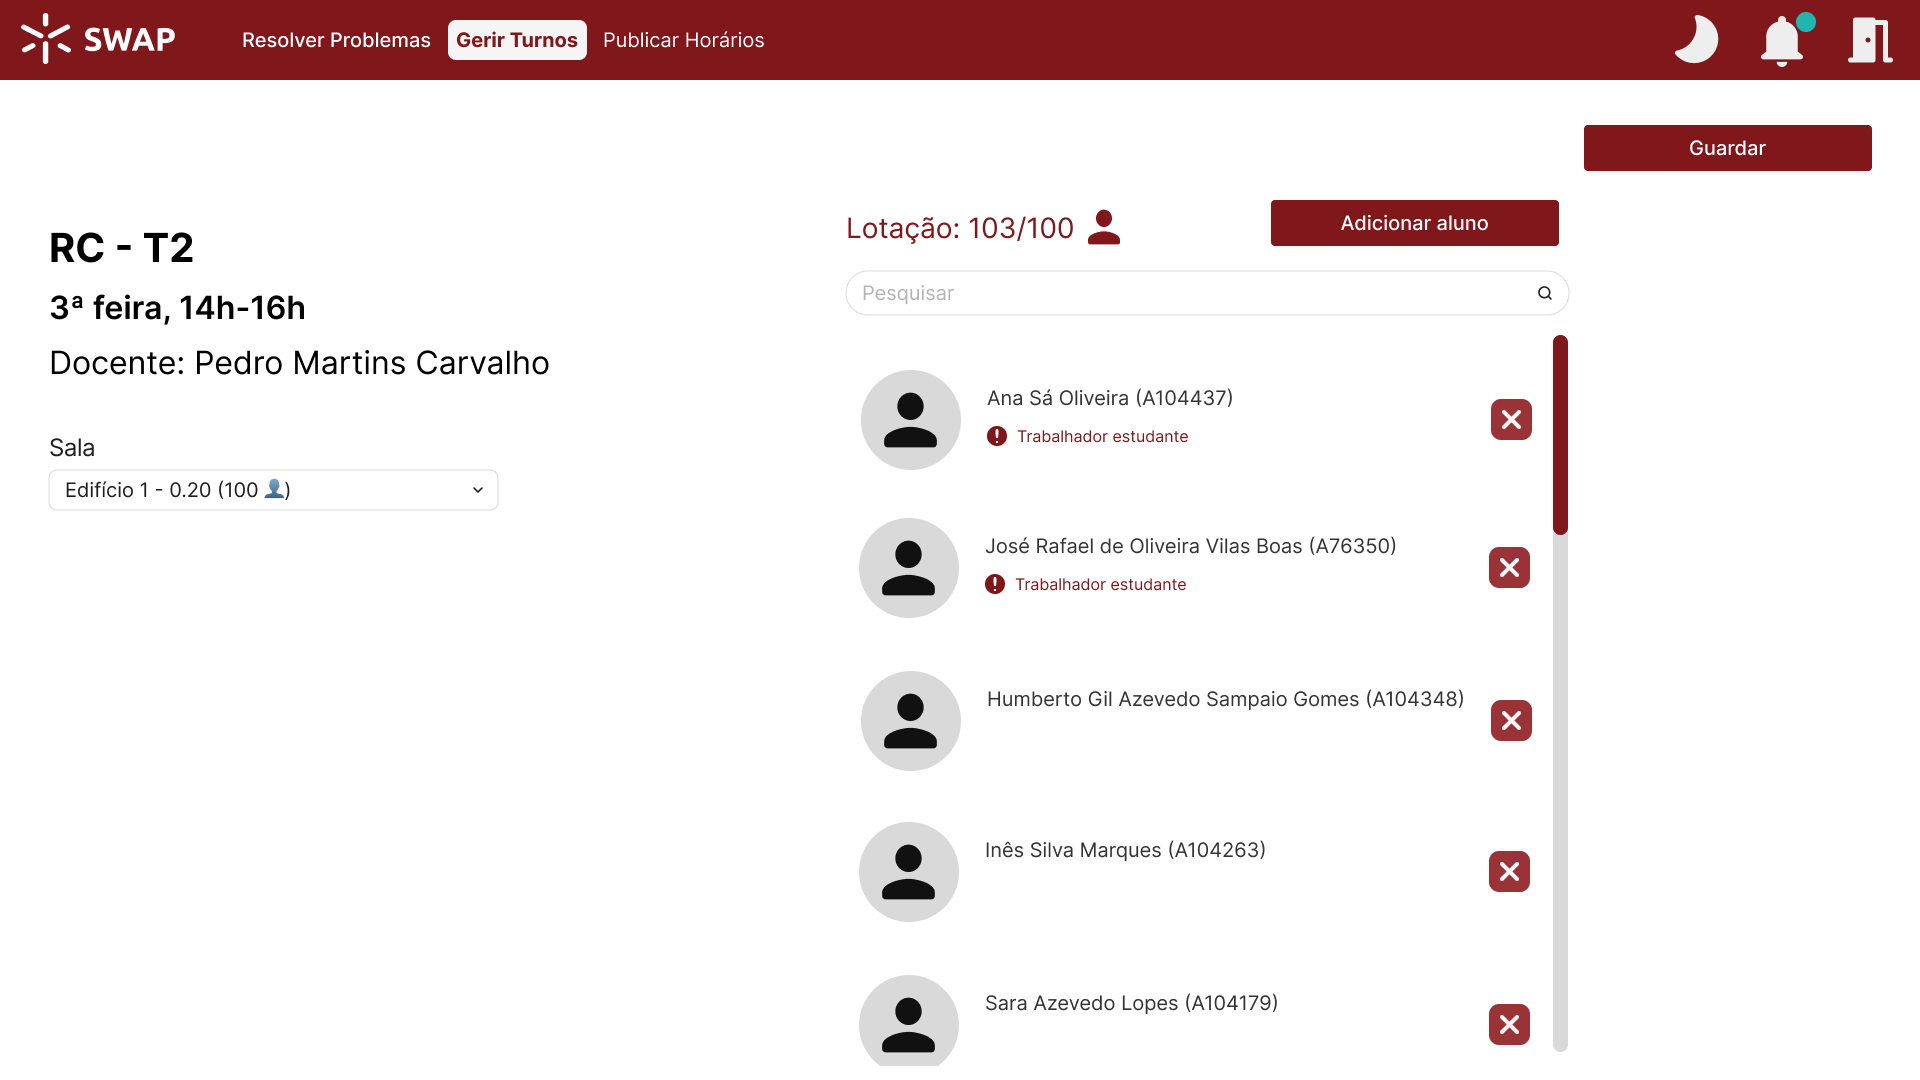
\includegraphics[width=0.8\textwidth]{res/prototype/gerir-turno.png}
    \caption{Captura de ecrã do protótipo da página ``Gerir Turno''.}
    \label{gerir-turno}
\end{figure}

Como se pode observar, do lado esquerdo da página, é possível ver alguma informação sobre o turno
selecionado para modificação, e também uma lista de \emph{dropdown} para escolha da sala do turno.
Esta lista deve apenas apresentar salas com capacidade suficiente para o turno. Ademais, devem ser
apresentadas em primeiro lugar as salas livres, e só depois opções de troca de sala com outros
turnos (que não façam com que esses turnos fiquem sobrelotados). Por último, o segundo critério de
ordenação deve ser a capacidade das salas:

\begin{figure}[H]
    \centering
    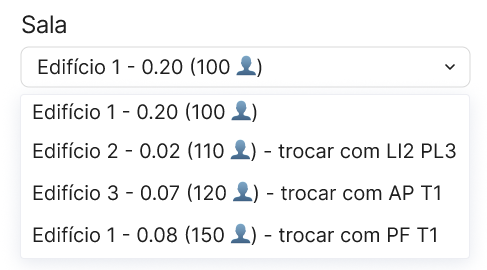
\includegraphics[width=0.5\textwidth]{res/prototype/gerir-turno-dropdown-salas.png}
    \caption{Lista de \emph{dropdown} para a definição da sala de um turno.}
    \label{gerir-turno-dropdown-salas}
\end{figure}

Com esta ordenação da lista, como é mais provável que o diretor de curso selecione uma das primeiras
opções, é mais provável que escolha uma sala que não cause distúrbios a outros turnos (não exija
outras mudanças de sala) e que não tenha uma capacidade excessiva, deixando as salas maiores para
turnos que realmente precisem delas. Para a escolha da sala, foi decidido que uma lista de
\emph{dropdown} seria utilizada, visto que apenas era necessário que o diretor de curso escolhesse
uma sala válida, e não uma sala em específico. Deste modo, é possível apresentar as opções de troca
de uma forma mais simples, sem adicionar complexidade à interface.

Do lado direito da página, é possível gerir o conjunto de alunos inscrito no turno. Em primeiro
lugar, está disponível uma barra de pesquisa, que permite filtrar que alunos devem ser apresentados,
permitindo uma melhor observabilidade dos conteúdos da página, especialmente em turnos de maior
dimensão. Ademais, encontra-se associado um botão a cada aluno, que o remove do turno. No protótipo
em Figma, um clique neste botão não se reflete na remoção do aluno da lista, uma vez que isso
levaria à necessidade da prototipagem um número excessivamente elevado de estados. No entanto, um
efeito observável da interação com este botão é a apresentação da mensagem abaixo:

\begin{figure}[H]
    \centering
    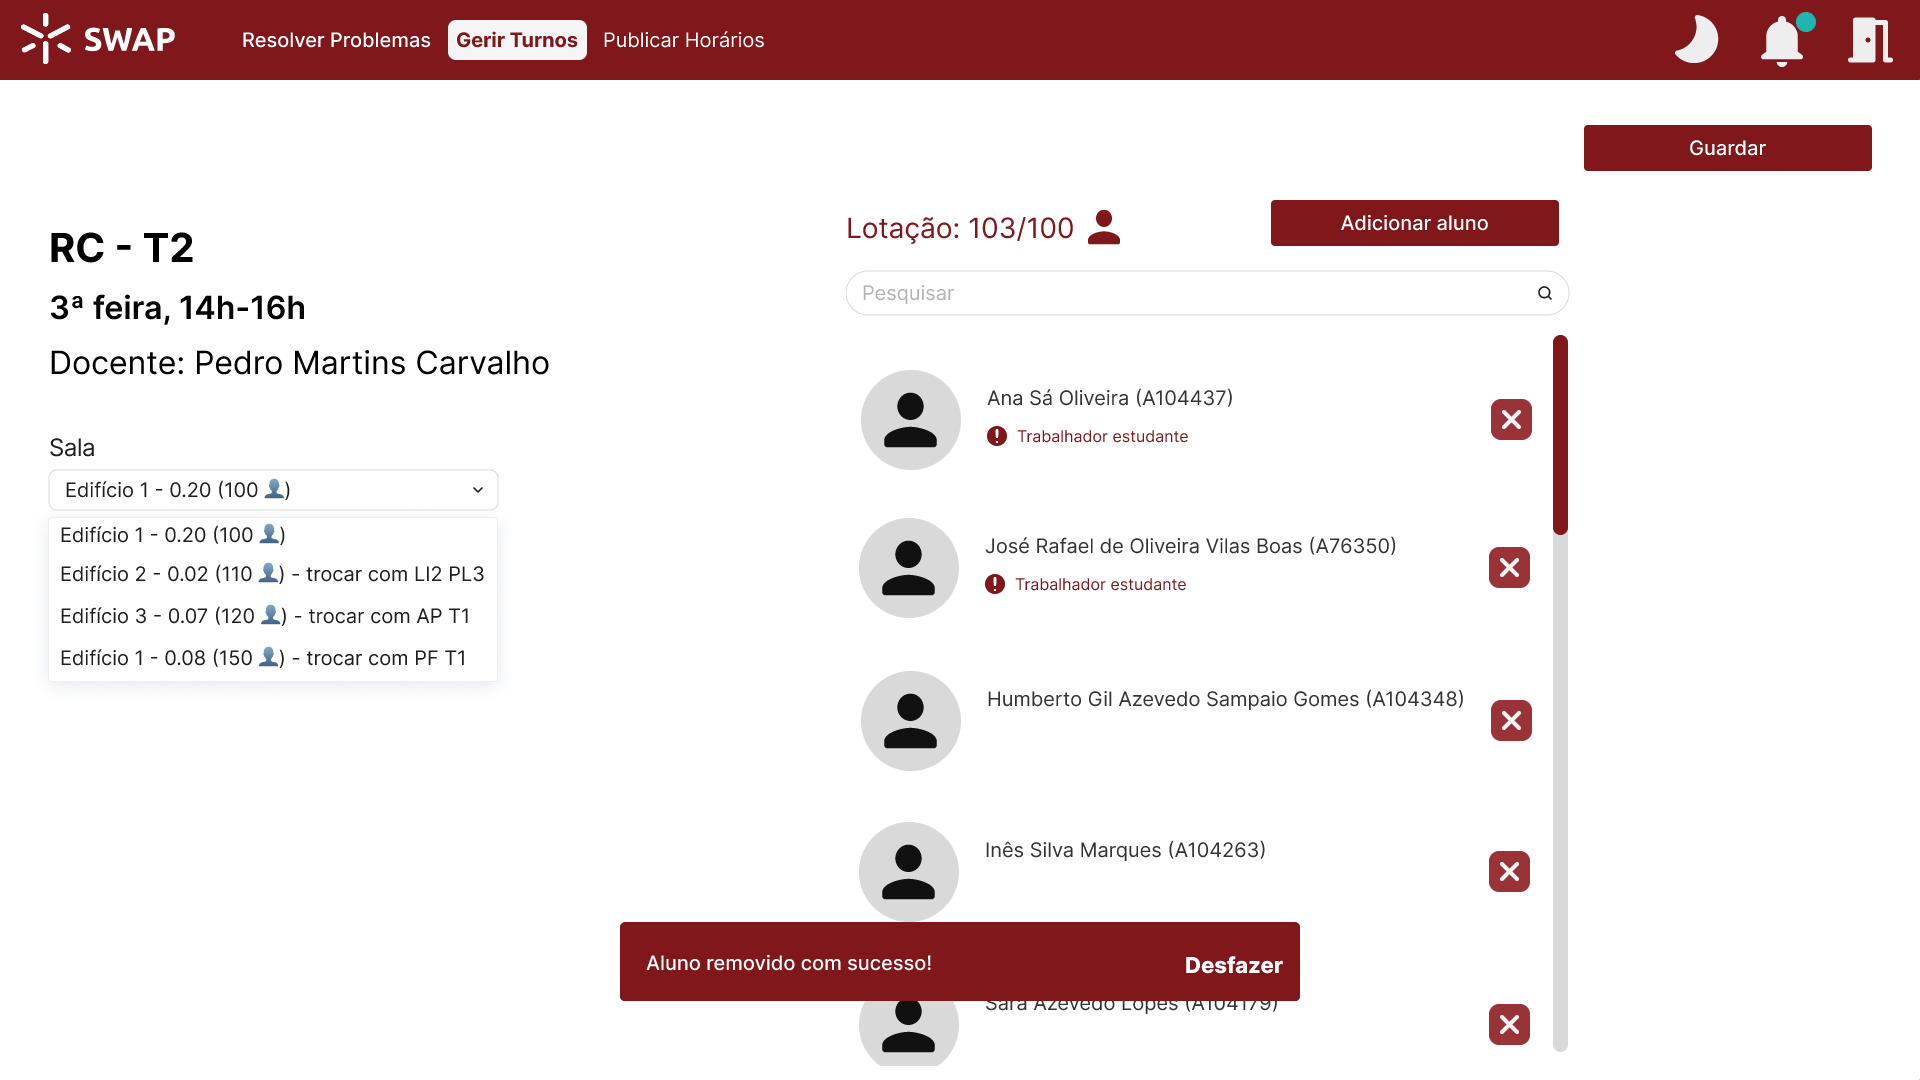
\includegraphics[width=0.8\textwidth]{res/prototype/gerir-turno-desfazer.png}
    \caption{
        \onehalfspacing
        Captura de ecrã do protótipo da página ``Gerir Turno'' com a opção de desfazer a remoção de
        um aluno do turno.
    }
    \label{gerir-turno-desfazer}
\end{figure}

Para o diretor de curso minimizar o seu tempo a utilizar a aplicação, como é descrito pelo perfil
do José, a opção de desfazer a ação de remover um aluno surge instantaneamente após a sua execução,
e o diretor não tem de procurar esse aluno para o voltar a adicionar.

Por outro lado, para adicionar um aluno ao turno, o utilizador pode clicar no botão
``Adicionar aluno'', que abrirá o diálogo abaixo, onde o utilizador poderá procurar um novo aluno
para adicionar ao turno:

\begin{figure}[H]
    \centering
    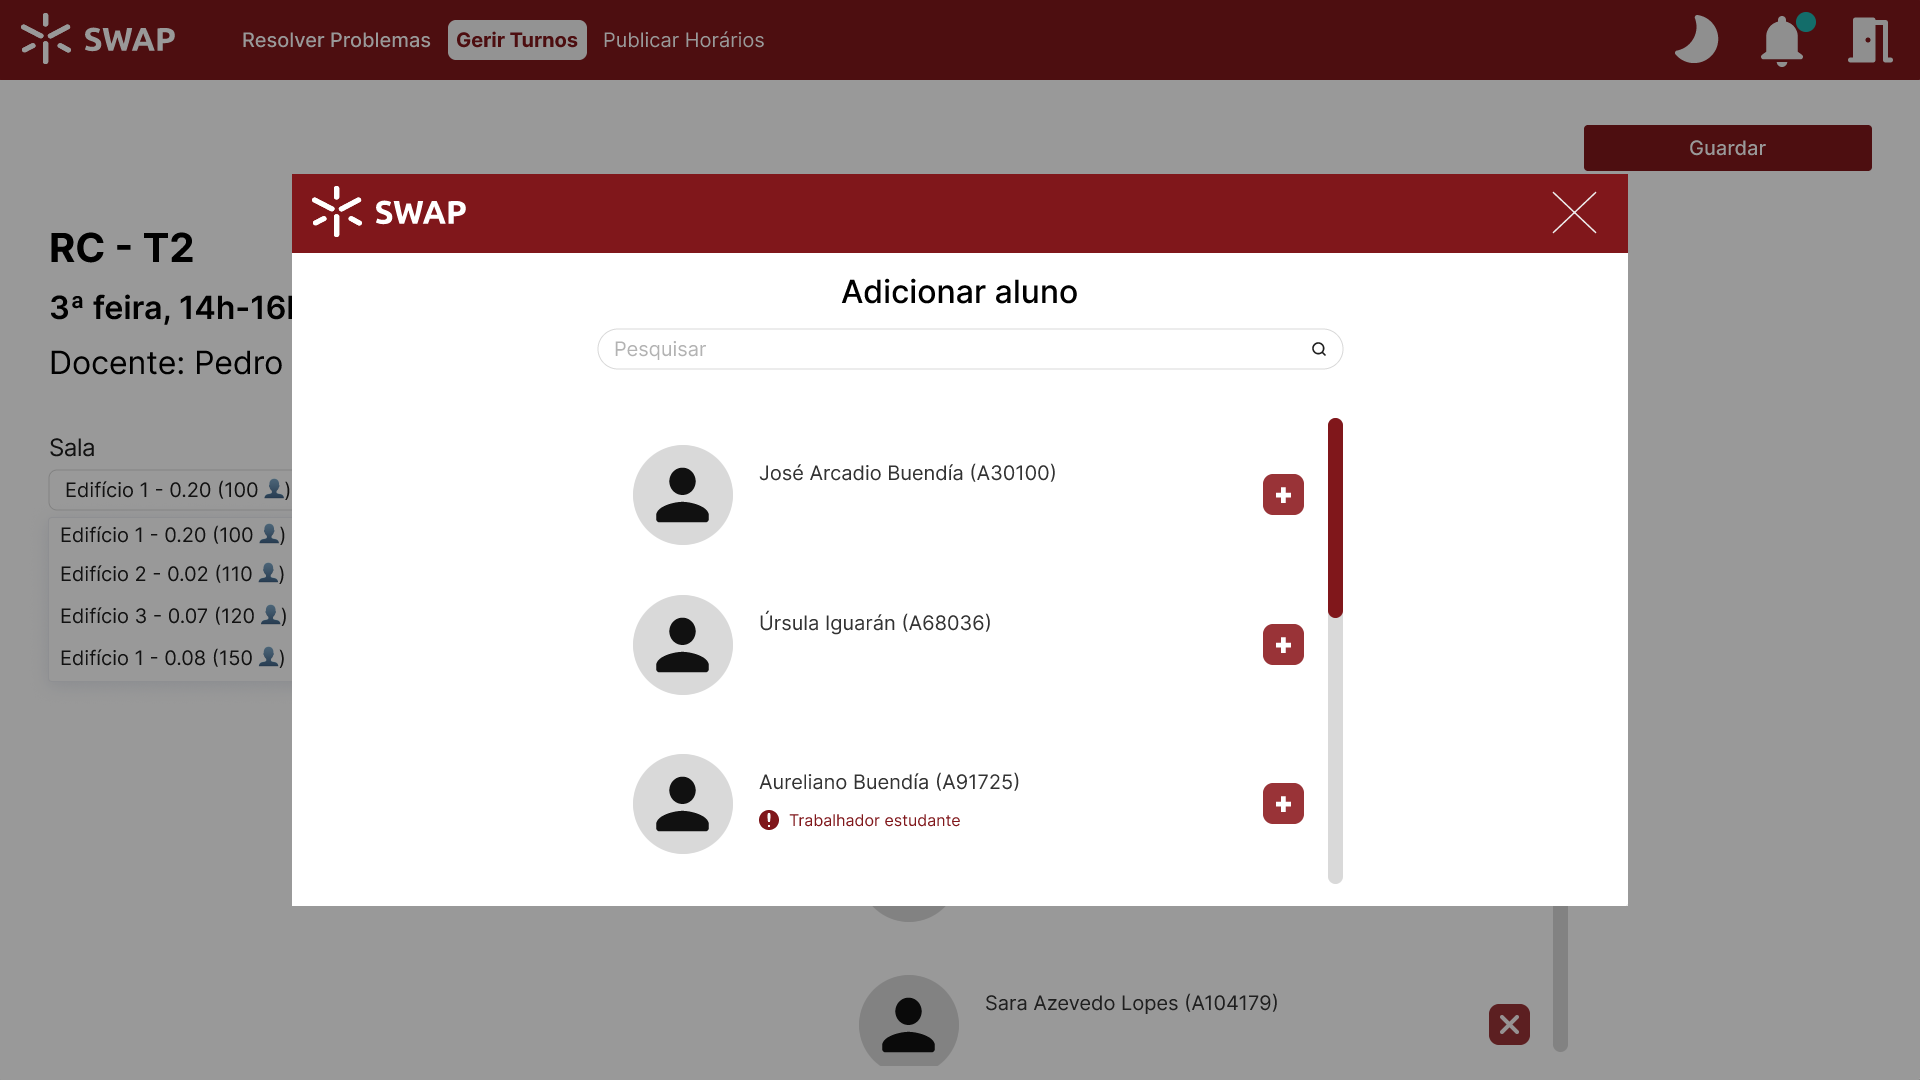
\includegraphics[width=0.8\textwidth]{res/prototype/gerir-turno-adicionar-aluno.png}
    \caption{
        \onehalfspacing
        Captura de ecrã do diálogo para adição de um aluno a um turno na página ``Gerir Turno''.
    }
    \label{gerir-turno-desfazer-adicionar-aluno}
\end{figure}

Quando um aluno é adicionado com um clique num dos botões ``+'', este diálogo será fechado e será
apresentada uma mensagem semelhante à da figura \ref{gerir-turno-desfazer}, permitindo ao utilizador
facilmente desfazer a sua ação, contribuindo para a recuperabilidade da interface.

\subsection{Página ``Publicar Horários''}

Quando o diretor de curso completa as alterações que deseja aos horários, pode publicá-los, um
processo descrito no cenário 1. Para o fazer, pode utilizar a página ``Publicar Horários'', cujo
protótipo é apresentado abaixo:

\begin{figure}[H]
    \centering
    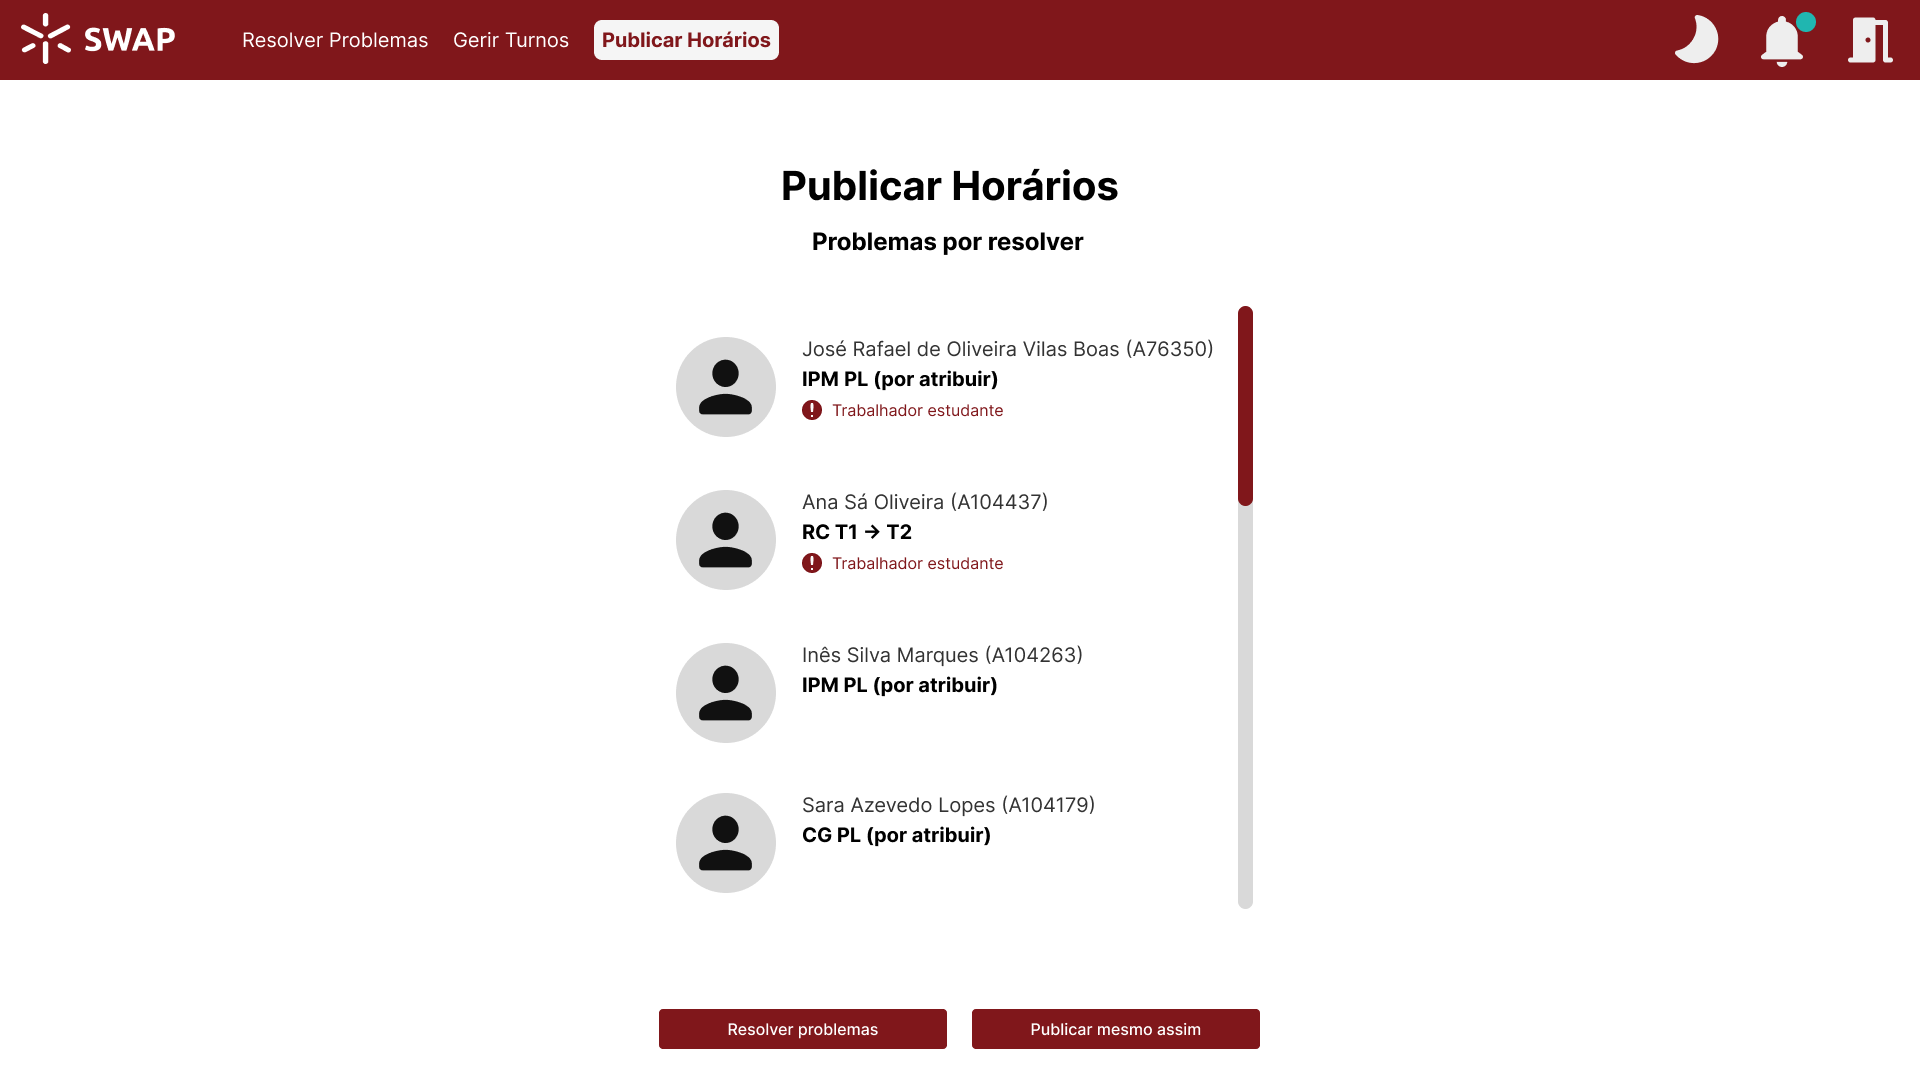
\includegraphics[width=0.8\textwidth]{res/prototype/publicar-horarios.png}
    \caption{Captura de ecrã do protótipo da página ``Publicar Horários''.}
    \label{publicar-horarios}
\end{figure}

Nesta página, antes do diretor de curso publicar os horários, é-lhe apresentada uma lista dos
problemas ainda por resolver. É de notar que o sistema não impede que o diretor de curso publique
horários com turnos por atribuir e pedidos de troca por satisfazer (o diretor é livre para o fazer
se assim o desejar), mas confirma diversas vezes que essa é a sua intenção: primeiro é apresentada
esta lista de problemas por resolver, e se o diretor decidir publicar os horários mesmo assim, o
seguinte diálogo de confirmação é apresentado:

\begin{figure}[H]
    \centering
    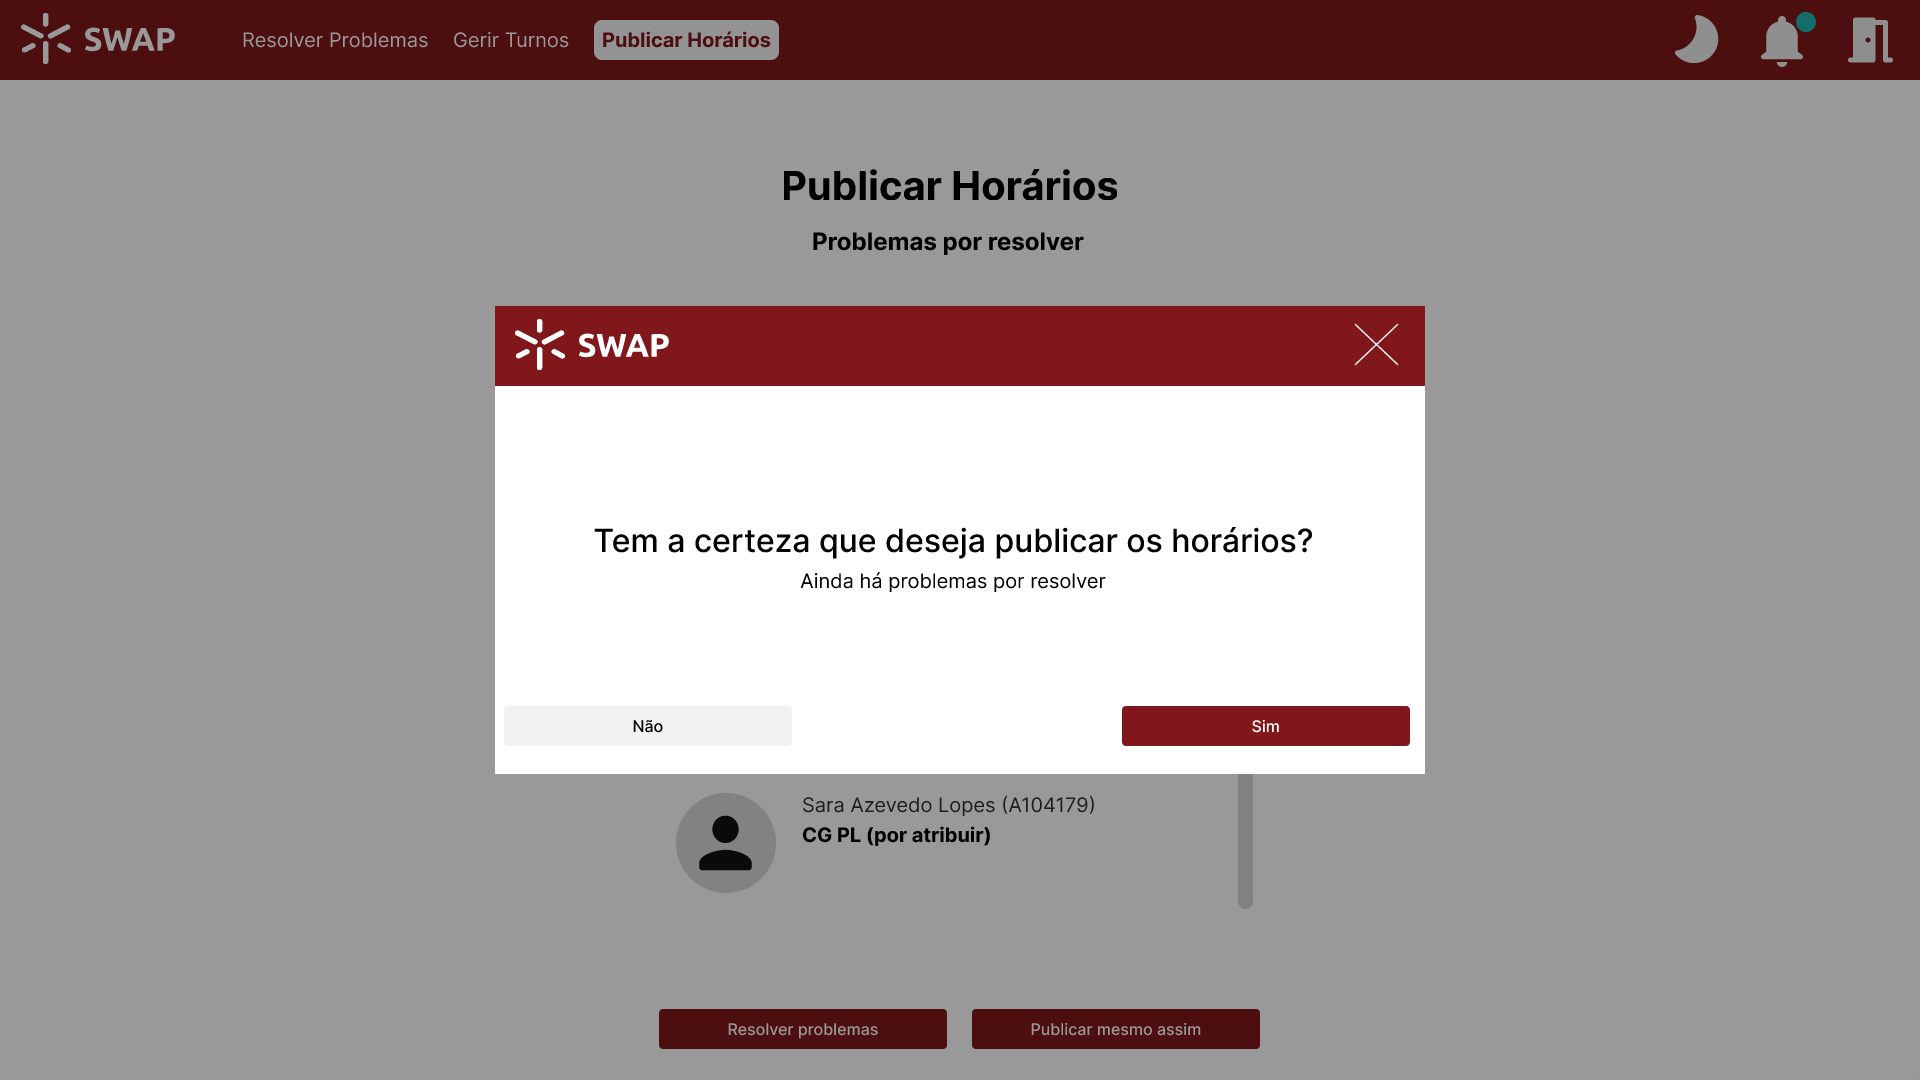
\includegraphics[width=0.8\textwidth]{res/prototype/dialogo-confirmacao-publicacao.png}
    \caption{Diálogo para confirmação da publicação dos horários na página ``Publicar Horários''.}
    \label{dialogo-confirmacao-publicacao}
\end{figure}

Estas confirmações seguem o princípio do esforço proporcional, sendo necessário um maior esforço
para executar estas ações irreversíveis, como a publicação de horários. Caso o utilizador não deseje
publicar os horários, pode fechar este diálogo e carregar no botão ``Resolver problemas'', ou num
dos problemas apresentados, o que o redirecionará para a página ``Resolver Problemas''. Por outro
lado, caso o utilizador decida publicar os horários, uma mensagem de confirmação é apresentada, para
dar \emph{feedback} ao utilizador do sucesso desta operação definitiva:

\begin{figure}[H]
    \centering
    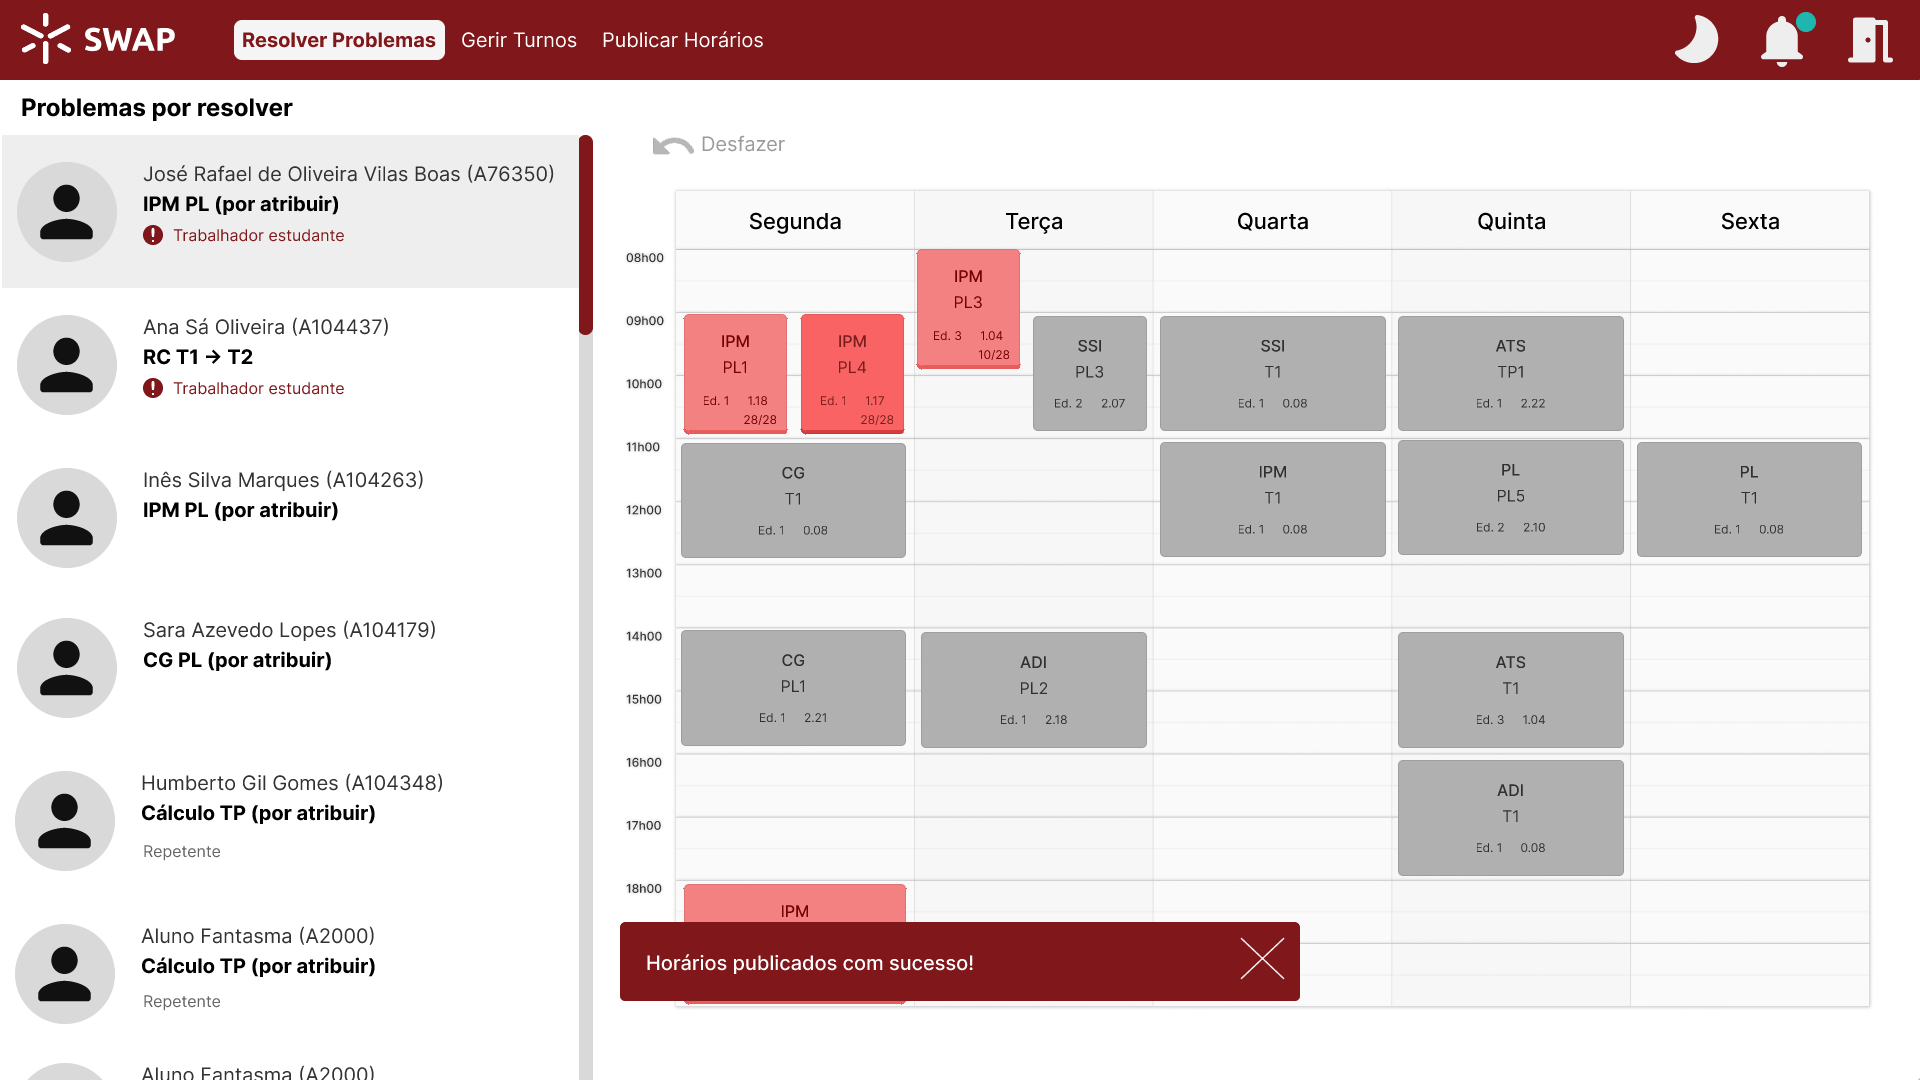
\includegraphics[width=0.8\textwidth]
        {res/prototype/resolver-problemas-toast-sucesso-publicao.png}
    \caption{
        \onehalfspacing
        Captura de ecrã do protótipo da página ``Resolver Problemas'' com a confirmação de sucesso
        na publicação de horários.
    }
    \label{resolver-problemas-toast-sucesso-publicao}
\end{figure}

\subsection{Página ``Notificações do Diretor de Curso''}

Esta página, semelhante à página ``Notificações do Aluno'', permite que o diretor de curso veja as
notificações de eventos que lhe possam ser relevantes:

\begin{figure}[H]
    \centering
    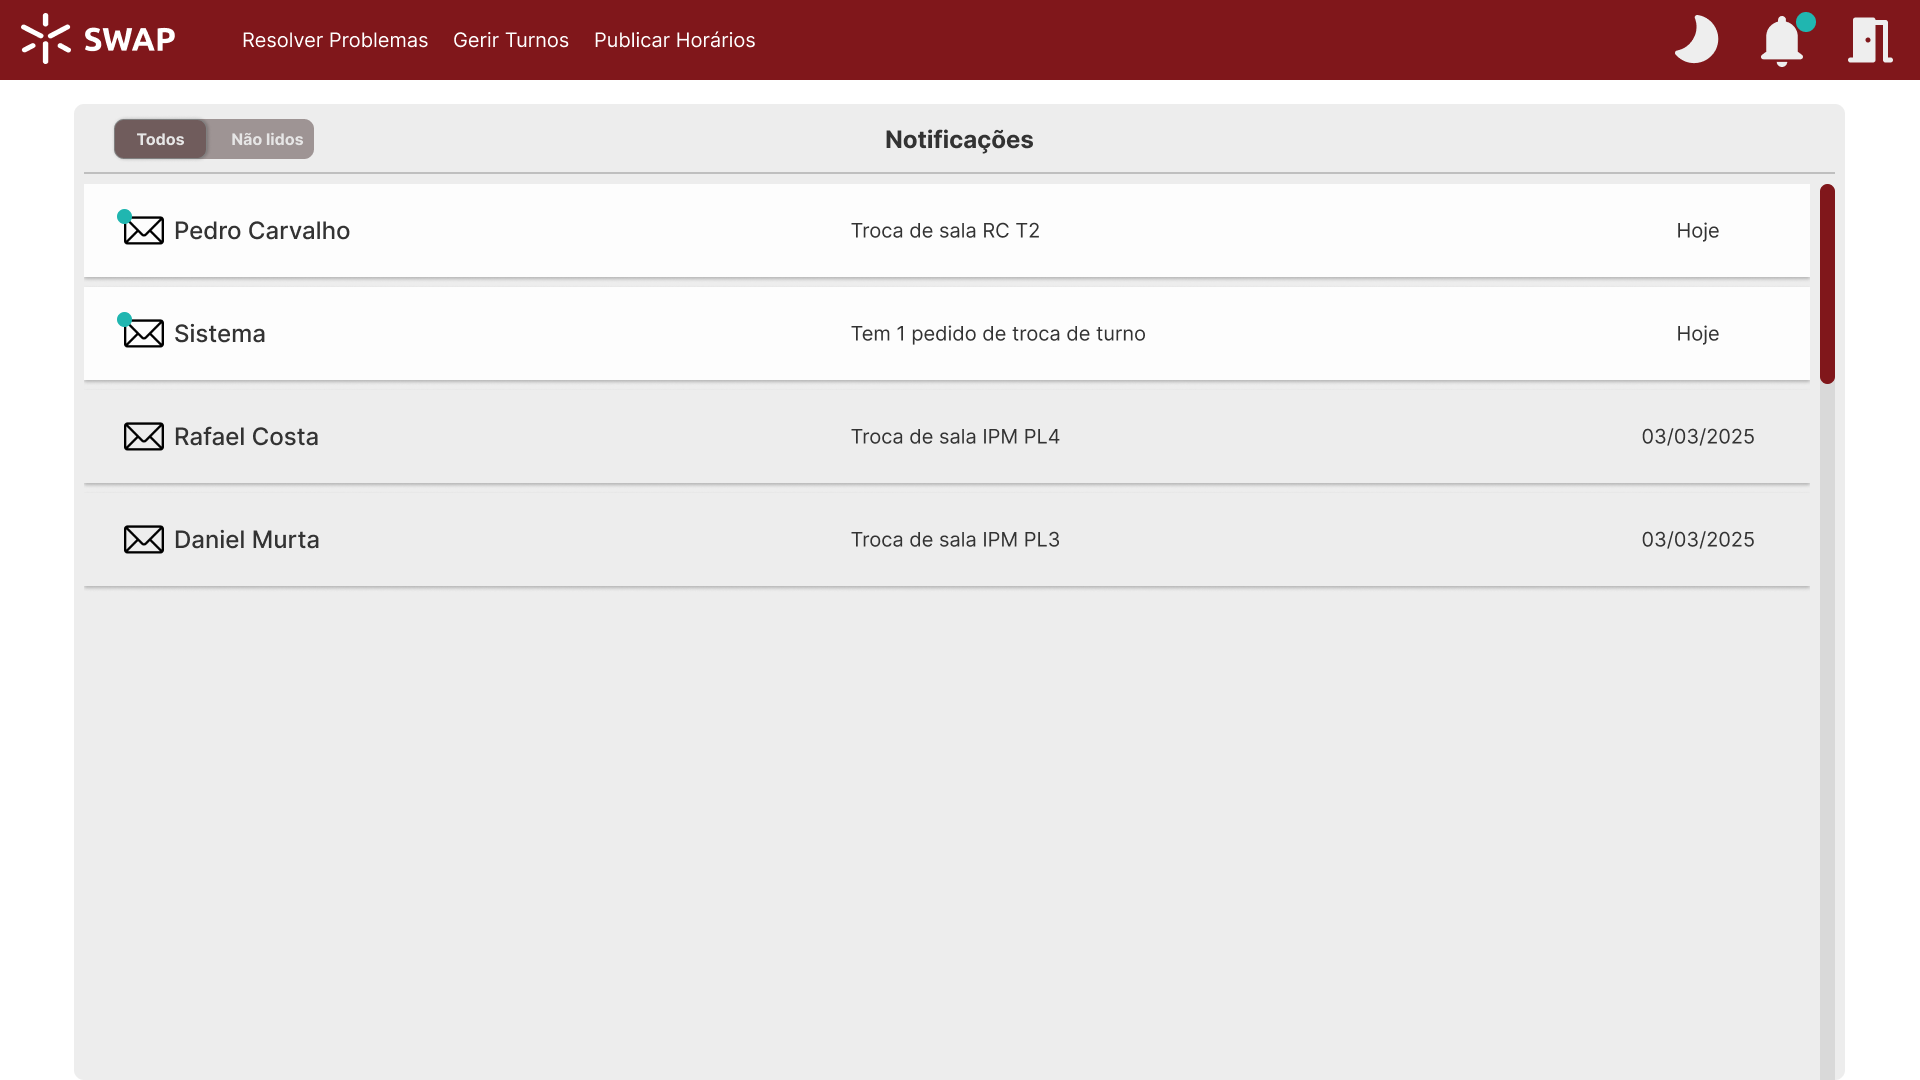
\includegraphics[width=0.8\textwidth]{res/prototype/notificacoes-diretor.png}
    \caption{Captura de ecrã do protótipo da página ``Notificações do Diretor de Curso''.}
    \label{notificacoes-diretor}
\end{figure}

Os tipos de notificação possíveis são os seguintes:

\begin{itemize}
    \item Pedido de troca de sala por parte de um docente (cenário 2);
    \item Pedidos de troca de turnos por parte de estudantes (cenários 3 e 4). Os pedidos são
        agrupados (por exemplo, ``Tem N pedidos de troca de turno'') para que estes, devido ao maior
        número de alunos, não ultrapassem em número os pedidos de docentes, o que poderia fazer com
        que estes últimos não fossem vistos pelo diretor;
\end{itemize}

Ao contrário do que acontecia na página ``Notificações do Aluno'', o diretor de curso faz mais com
uma notificação do que ser informado do seu conteúdo: precisa de agir sobre ela. Logo, quando
sobrevoa o cursor sobre uma notificação, os seguintes botões devem aparecer no seu lado direto:

\begin{figure}[H]
    \centering
    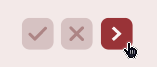
\includegraphics[width=0.3\textwidth]{res/prototype/notificacoes-diretor-hover.png}
    \caption{Botões que surgem quando uma notificação é sobrevoada pelo cursor.}
    \label{notificacoes-diretor-hover}
\end{figure}

Da esquerda para a direita, estes permitem marcar a notificação como resolvida, marcá-la como algo
que não será resolvido, e ir para a página onde pode ser resolvida. Por exemplo, quando se clica num
destes últimos botões associado a um pedido de troca de sala, o utilizador será redirecionado para a
página ``Gerir Turno'' do turno correspondente. As notificações em diferentes estados são
representadas em diferentes tons de cinza. A figura seguinte apresenta, de cima para baixo, duas
notificações por ler, uma notificação por tratar, e uma notificação tratada ou rejeitada:

\begin{figure}[H]
    \centering
    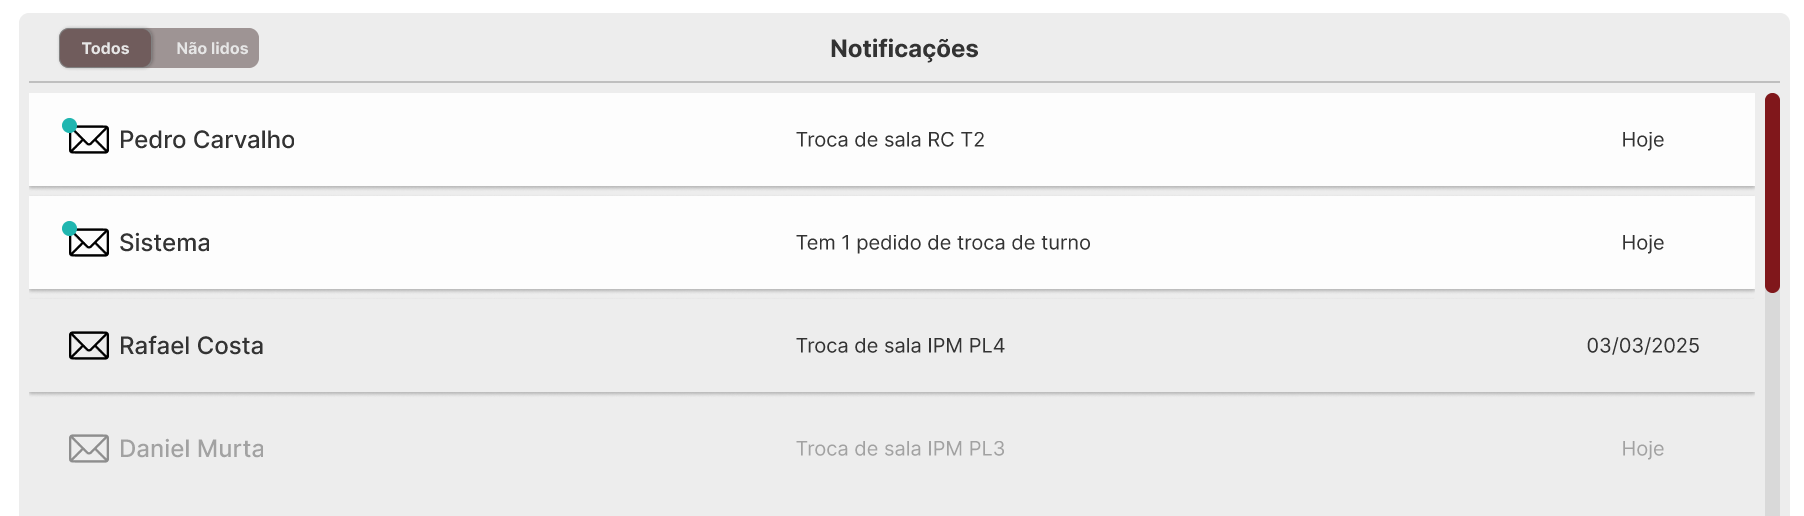
\includegraphics[width=0.8\textwidth]{res/prototype/notificacoes-diretor-cor.png}
    \caption{Cores das notificações do diretor de curso conforme o seu estado.}
    \label{notificacoes-diretor-cor}
\end{figure}

\section{Mapa de Navegação}

\section{Avaliação Heurística}

\section{Conclusão e Trabalho Futuro}

\begingroup
\section{Bibliografia}
\renewcommand{\section}[2]{}

\begin{thebibliography}{9}
    \bibitem{figma}
        "Figma: Collaborative Interface Design Tool."{}. Figma. Accessed: Mar. 13, 2025. [Online.]
        Available: \url{https://www.figma.com/}
    \bibitem{nielsen}
        "10 Usability Heuristics for User Interface Design". Nielsen Norman Group.
        Accessed: Mar. 13, 2025. [Online.] Available:
        \url{https://www.nngroup.com/articles/ten-usability-heuristics/}
    \bibitem{material-icons}
        "Material Symbols \& Icons"{}. Google Fonts. Accessed: Mar. 14, 2025. [Online.] Available:
        \url{https://fonts.google.com/icons}
\end{thebibliography}
\endgroup

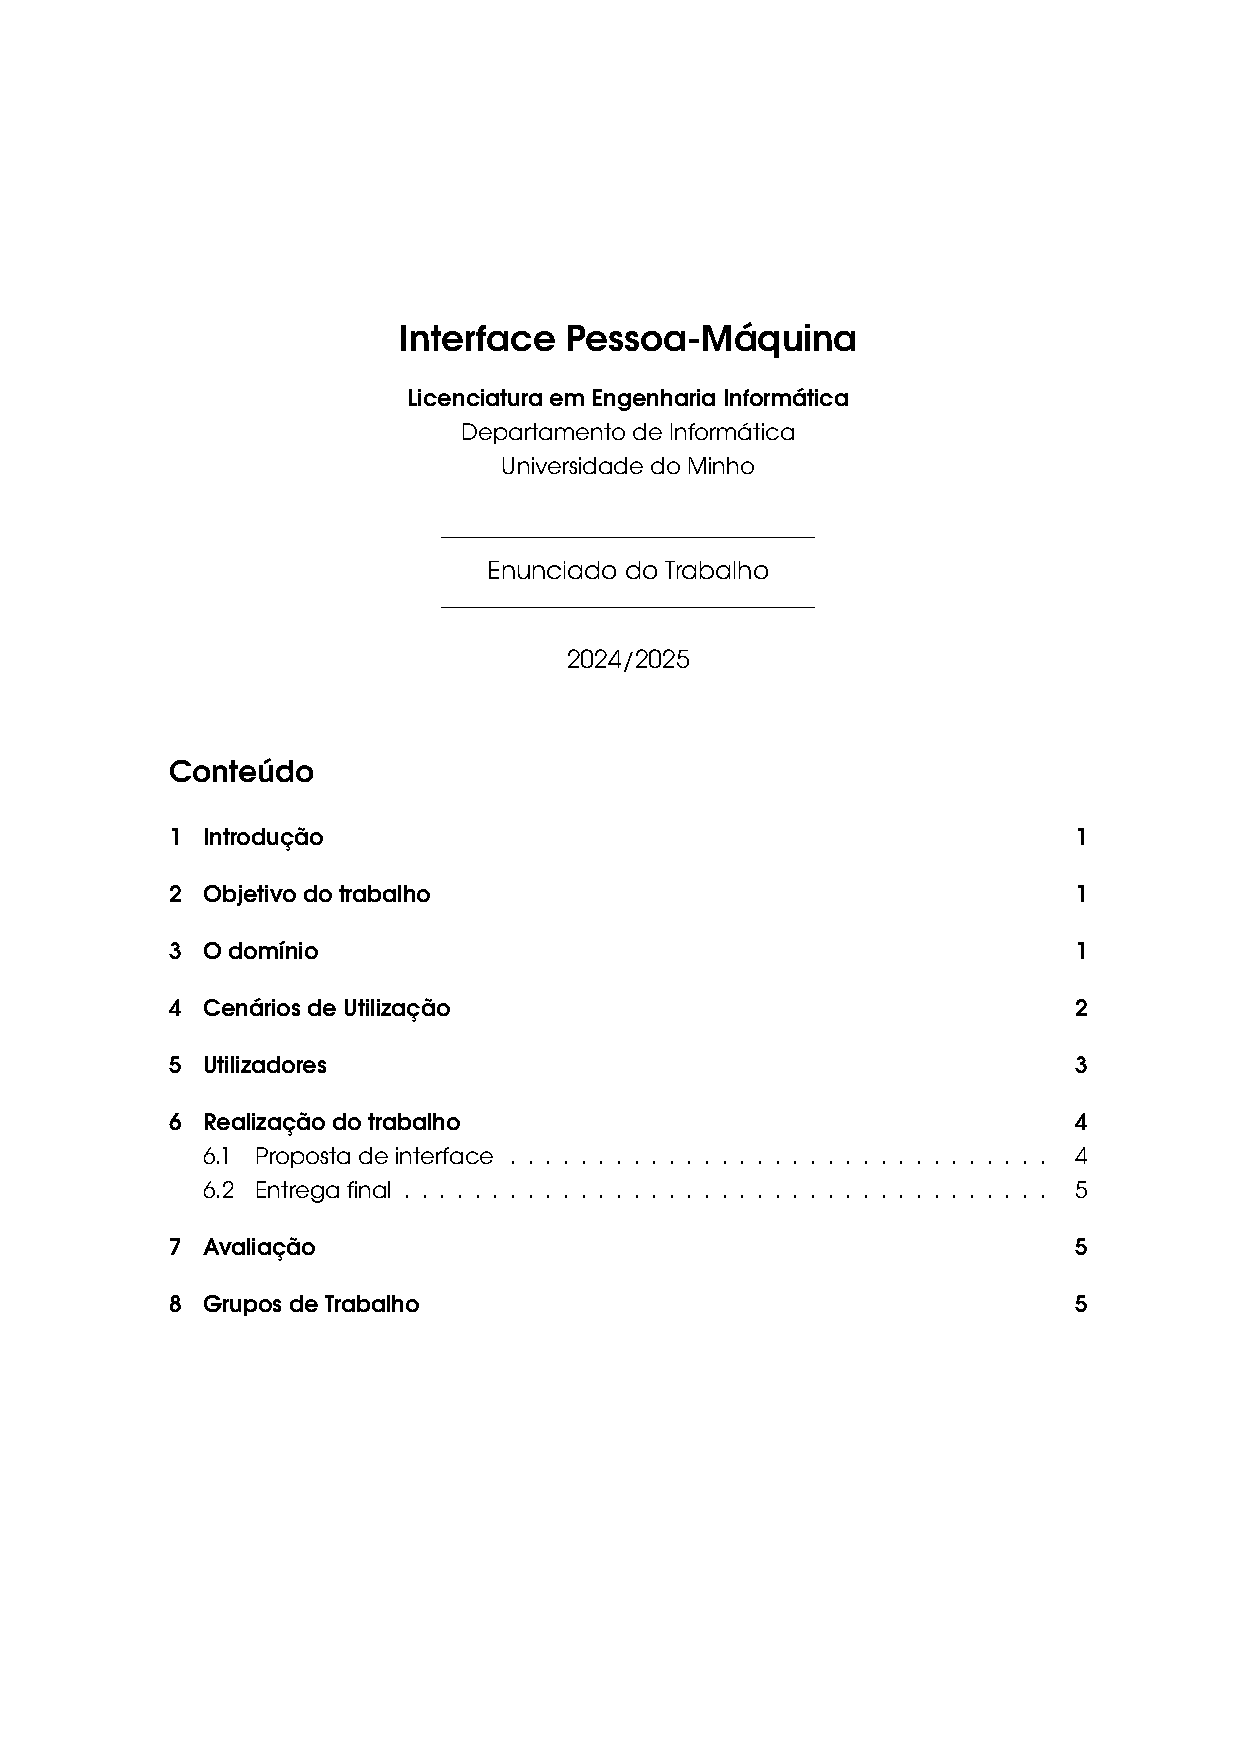
\includepdf[pages=1,pagecommand=\section{Anexo -- Enunciado do Trabalho}\thispagestyle{empty}]
    {../Assignment.pdf}
\includepdf[pages=2-]{../Assignment.pdf}

\end{document}
